\documentclass[11pt]{article}
\usepackage[margin=1in]{geometry}
\usepackage{amsmath,amssymb,amsthm,mathtools,booktabs,array}
\usepackage[T1]{fontenc}
\usepackage{lmodern}
\usepackage{microtype}
\usepackage{pgfplots}
\usepgfplotslibrary{groupplots}
\pgfplotsset{compat=1.18}
\definecolor{benchmark}{HTML}{B65A34}
\definecolor{eventaware}{HTML}{187B80}
\usepackage[colorlinks=true,linkcolor=blue,urlcolor=blue]{hyperref}
\definecolor{prototypeoriginal}{HTML}{7C3AED}
\definecolor{prototypeaware}{HTML}{059669}
\definecolor{prototypehazard}{HTML}{F59E0B}
\definecolor{prototypeevent}{HTML}{DC2626}
\newcommand{\E}{\mathbb E}
\newcommand{\Prob}{\mathbb P}
\newcommand{\1}{\mathbf 1}
\newcommand{\dd}{\mathrm d}
\newcommand{\F}{\mathcal F}
\newcommand{\G}{\mathcal G}
\newcommand{\A}{\mathcal A}
\newtheorem{proposition}{Proposition}
\title{Event-Aware Market Making in Prediction Markets\\\large Anticipated Information and Stale-Quote Execution}
\author{Model specification}
\date{October 14, 2026}
\begin{document}
\maketitle
\begin{abstract}
We specify an inventory-sensitive market maker for a binary prediction contract.
Fair value evolves through continuous diffusion, recurring unscheduled news,
and a single anticipated information event with a time-dependent arrival hazard.
Information shocks may execute against outstanding quotes before cancellation,
so news affects both inventory risk and the immediate economics of quoting.
The control problem reduces to two coupled Hamilton--Jacobi--Bellman
partial integro-differential equations, corresponding to the anticipated event
being pending or completed. We give the event operator, terminal conditions,
a qualified spread-widening result, and a reproducible Monte Carlo comparison
with a constrained diffusion benchmark. The numerical experiment measures
performance under synthetic news and execution assumptions.
\end{abstract}

\section{Scope and modeling conventions}
This document formalizes the event-aware market-making framework developed in the
\href{https://chatgpt.com/s/t_6ad02e77e93c8191b242a759e44d98b6}{shared research discussion}.
Its defining change is to distinguish \emph{when information arrives} from
\emph{how much uncertainty it resolves}, and to allow the resulting price jump
to trade against a stale quote. The anticipated event occurs at most once;
unscheduled news can recur.

The baseline uses certain execution of a crossed stale quote, a fixed trade
size, and no fees. Quotes are predictable: the maker chooses them before
observing the information shock. After the shock and any stale execution,
the maker may reprice. Ordinary order arrivals convey no additional information
about the contract payoff in this specification.

We retain the source model's equations while making the following conventions
explicit: both news kernels preserve conditional mean; prices lie in $[0,1]$;
running event risk uses pre-event inventory; and unconditional variance matching
includes the probability that the one-shot event is still pending. Numerical
choices and empirical hypotheses below are distinguished from model identities.

\section{Prior work and relationship to this model}
\label{sec:prior}
\subsection{Direct foundation: prediction-market optimal control}
Feil and Nendel~\cite{feilnendel2026} provide the direct foundation: a bounded
martingale belief generated by a latent diffusion, fixed-size executions,
inventory-sensitive quoting, and running and terminal risk penalties.
Their Sections~2--3 develop the control problem and its reduced Bellman equation;
Example~2.1 supplies the logistic diffusion behind the factor $p(1-p)$ used here.
The decomposition $U=x+qp+V$ retains that structure.

There are material differences. Their model has continuous pre-resolution
beliefs, a finite inventory grid, general time- and belief-dependent execution
intensities, and quotes in $[0,1]^2$. Our straddling constraint $b\le p\le a$
and symmetric exponential intensities are additional restrictions. Their payoff
is revealed immediately after the trading horizon, explaining the residual
settlement penalty. Their classical-solution and verification results do not
automatically extend to our nonlocal, regime-switching equations with atomic
kernels and discontinuous fill indicators.

\subsection{Broader inventory and adverse-selection literature}
Avellaneda and Stoikov~\cite{avellanedastoikov2008} establish a canonical
inventory-based quoting framework with diffusive prices and quote-dependent
Poisson executions, including exponential arrival intensities. This is the
broader lineage of our ordinary-fill Hamiltonian. Their exponential-utility
criterion differs from the additive inventory penalties used here; their
closed-form approximations should not be imported unchanged into this model.

Cartea, Jaimungal, and Penalva~\cite{cartea2015}, particularly Chapter~10 and
Section~10.4, provide broader context for stochastic-control market making and
adverse selection. We cite this as methodological background, not as the source
of our particular one-shot event operator. The present model represents adverse selection
through a specified news-triggered crossing rule rather than estimating a full
model of informed order flow.

\subsection{Empirical motivation for anticipated information}
Frino and Hill~\cite{frinohill2001} study scheduled macroeconomic announcements
in Australian futures markets. They report significant spread widening during
the 20 seconds before announcements and the 30 seconds afterward. This supports
investigating time-localized quoting responses, but does not establish our
prediction-market calibration or certain-pickoff assumption.

Siikanen, Kanniainen, and Valli~\cite{siikanen2017} distinguish scheduled and
unscheduled company announcements using NASDAQ Nordic order books. They find
announcement-related changes in liquidity and emphasize that multi-level depth
can behave differently from the best bid--ask spread; scheduled announcements
can improve multi-level liquidity. Their findings motivate separate event
types and caution against interpreting wider spreads as a complete measure of
liquidity deterioration. Neither empirical study proves this model's comparative
statics or measures its proposed economic advantage.

\subsection{Model extensions}
Relative to the direct diffusion foundation, this model adds recurring unscheduled
news, a one-shot anticipated event with survival-dependent arrival, and
execution at pre-event quotes after fair value changes. The risk criterion
extends the diffusion variance charge to predictable quadratic variation.
These additions yield the coupled equations below and make event exposure
enter quote optimization directly through $\G^K_{b,a}$.

The event operator depends on the controls and changes inventory, unlike a
quote-independent jump operator. The pending/completed state prevents repeat
arrivals of the same anticipated release. These features describe the model's
scope; they are not claims of priority over the entire market-microstructure literature.
The two-controller numerical comparison below measures the combined effect
of these extensions; isolating timing information remains a further test.

\section{State, fair value, and information arrivals}
\subsection{Contract and state variables}
The contract pays $Y\in\{0,1\}$ at resolution. Over a trading horizon $[0,T]$,
define the fair probability by
\begin{equation}
 p_t=\E[Y\mid\F_t]\in[0,1].
\end{equation}
The maker holds cash $X_t$ and inventory $Q_t\in\Delta\mathbb Z$, where
$\Delta>0$ is the quantity executed per fill. Let
\begin{equation}
 S_t=\1_{\{\tau\le t\}}\in\{0,1\}
\end{equation}
indicate whether the anticipated information event at time $\tau$ has occurred.
The Markov state is $(t,X_t,p_t,Q_t,S_t)$. The horizon may precede payoff
resolution; conditional expected terminal inventory value is then $Q_Tp_T$.
If $T$ is resolution itself, $p_T=Y$ and residual Bernoulli variance vanishes.

\subsection{Continuous variation and unscheduled news}
Between information events,
\begin{equation}
 \dd p_t=\sigma(t,p_t)\dd W_t,
 \qquad \sigma(t,p)=\bar\sigma(t,p)p(1-p).
\end{equation}
Assume coefficients are regular enough for a well-defined process that stays
in $[0,1]$. Unscheduled shocks arrive with intensity $\lambda_u(t,p)$.
At a shock, the new probability has kernel $K_u(\dd p'\mid p)$ supported on
$[0,1]$, with
\begin{equation}
 \int p'K_u(\dd p'\mid p)=p,
 \qquad v_u(p)=\int(p'-p)^2K_u(\dd p'\mid p).
\end{equation}
Thus neither diffusion nor unscheduled news creates predictable fair-value
drift. Kernels may be extended to depend on time, with corresponding changes
to notation.

\subsection{The anticipated event}
Let $F$ be the arrival-time distribution, with density $f$ on the modeled
window. Conditional on survival, its hazard is
\begin{equation}
 h(t)=\frac{f(t)}{1-F(t)},\qquad
 \Prob(\tau\in[t,t+\dd t]\mid\tau>t)=h(t)\dd t+o(\dd t).
\end{equation}
The actual event intensity is $(1-S_{t-})h(t)$. At arrival, $S$ changes
from $0$ to $1$ and never changes back. The probability transition kernel
$K_s$ satisfies
\begin{equation}
 \int p'K_s(\dd p'\mid p)=p,
 \qquad v_s(p)=\int(p'-p)^2K_s(\dd p'\mid p).
\end{equation}
The subscript on $K_s$ denotes the scheduled/anticipated event type, whereas
the index on $V_s$ below denotes the regime $s\in\{0,1\}$.
We assume the time-only hazard is valid conditional on the full pre-event
state, so that the absence of the event does not itself require a drift update
to $p$. An event time informative about $Y$ would require a richer filtering model.

A finite hazard window generally leaves positive probability that the event
has not occurred by $T$:
\begin{equation}
 \Prob(\tau>T\mid\tau>t)=\exp\left(-\int_t^T h(u)\dd u\right).
\end{equation}
An event guaranteed by a finite deadline instead requires a divergent
integrated hazard or an atom, treated as a discrete event condition.

\subsection{A mean-preserving two-point kernel}
For either event type, a convenient choice is $K_\rho$, $0\le\rho\le1$:
\begin{equation}
 p'=\begin{cases}
 p^+=p+\rho(1-p),&\text{with probability }p,\\
 p^-=(1-\rho)p,&\text{with probability }1-p.
 \end{cases}
\end{equation}
Direct calculation gives
\begin{equation}
 \E[p'\mid p]=p,\qquad
 \E[(p'-p)^2\mid p]=\rho^2p(1-p).
\end{equation}
Use separate parameters $\rho_u$ and $\rho_s$ for the two event types.
$\rho=0$ produces no news and $\rho=1$ fully resolves the probability.
Mean-preserving kernels on $[0,1]$ are degenerate at $p=0$ and $p=1$.

\section{Quotes and execution}
\subsection{Admissible controls}
At state $(t,p,q,s)$, the maker posts bid $b$ and ask $a$ in an admissible set
$\A(p,q)$. A baseline price constraint is
\begin{equation}
 0\le b\le p\le a\le1.
 \label{eq:quotes}
\end{equation}
Define quote distances $\delta_b=p-b$ and $\delta_a=a-p$.
If the experiment requires continuous meaningful participation, impose a
maximum quote displacement $D$:
\begin{equation}
 0\le\delta_b\le\min(D,p),\qquad
 0\le\delta_a\le\min(D,1-p).
 \label{eq:cap}
\end{equation}
Otherwise endpoint quotes can serve as effective protection against pickoff.
The restriction that quotes straddle $p$ is an assumption of this model and limits how aggressively
the maker can skew to reduce inventory.

The analytical state space is $\Delta\mathbb Z$. For finite-grid computation,
choose inventory limits and explicitly disable any side that would violate
them. A disabled side has neither ordinary fills nor stale fills. All formulas
below are for active sides; the same availability mask must be applied to both
execution mechanisms at inventory boundaries. This is an implementation
convention, not an additional source-model assumption.

\subsection{Ordinary market orders}
Away from news events, ordinary fills have intensities
\begin{equation}
 \Lambda^b(\delta_b)=Ae^{-k\delta_b},\qquad
 \Lambda^a(\delta_a)=Ae^{-k\delta_a},\qquad A,k>0.
\end{equation}
More general side-specific intensities can replace these functions. The
exponential specification follows the classical quoting framework
of~\cite{avellanedastoikov2008}; the prediction-market foundation
in~\cite{feilnendel2026} permits more general intensities.
A bid fill sends $(x,q)$ to $(x-\Delta b,q+\Delta)$; an ask fill sends it
to $(x+\Delta a,q-\Delta)$. For a reduced value function $V_s$, write
\begin{align}
 \F_{b,a}[V_s](t,p,q)={}&
 \Lambda^b(p-b)\bigl[\Delta(p-b)+V_s(t,p,q+\Delta)-V_s(t,p,q)\bigr]
 \notag\\
 &+\Lambda^a(a-p)\bigl[\Delta(a-p)+V_s(t,p,q-\Delta)-V_s(t,p,q)\bigr].
 \label{eq:fills}
\end{align}

\subsection{Stale-quote execution at information events}
An information event first reveals $p'$. Before cancellation, a fast trader
executes one lot against any strictly crossed stale quote:
\begin{equation}
 I_b(p';b)=\1_{\{p'<b\}},\qquad I_a(p';a)=\1_{\{p'>a\}},\qquad
 q'=q+\Delta I_b-\Delta I_a.
\end{equation}
Equality does not trigger a stale fill. The two indicators cannot both be one
under \eqref{eq:quotes}. The associated cash is
$x'=x-\Delta b I_b+\Delta a I_a$.
Define the event operator on a post-event reduced value $W$ by
\begin{align}
 \G^K_{b,a}[W](t,p,q)=\int\Bigl[
 &W(t,p',q')+\Delta(p'-b)I_b(p';b)
 \notag\\[-2pt]
 &+\Delta(a-p')I_a(p';a)\Bigr]K(\dd p'\mid p).
 \label{eq:event}
\end{align}
Both execution markouts are nonpositive. The operator jointly updates fair
value, inventory, and the loss from stale execution.

For clarity, the total mark-to-market change at the event is
\begin{equation}
 x'+q'p'-(x+qp)
 =q(p'-p)+\Delta(p'-b)I_b+\Delta(a-p')I_a.
\end{equation}
The first term has conditional mean zero because $K$ is mean-preserving;
the remaining terms explain \eqref{eq:event}. This calculation accounts for
the simultaneous jump and fill without omitting their interaction.

\section{Risk criterion and cash reduction}
With no predictable atoms in event time, the predictable quadratic variation is
\begin{equation}
 \dd\langle p\rangle_t=c_{S_{t-}}(t,p_{t-})\dd t,
 \qquad
 c_s(t,p)=\sigma^2(t,p)+\lambda_u(t,p)v_u(p)+(1-s)h(t)v_s(p).
 \label{eq:variance}
\end{equation}
For $\gamma,\gamma_T\ge0$, the maker maximizes
\begin{equation}
 U_s(t,x,p,q)=\sup_{\pi}\E_{t,x,p,q,s}\left[
 X_T+Q_TY-\gamma\int_t^T Q_{u-}^2\dd\langle p\rangle_u
 -\gamma_TQ_T^2p_T(1-p_T)\right].
 \label{eq:objective}
\end{equation}
The running penalty prices exposure to fair-value variation, including jumps.
The terminal penalty prices residual payoff variance at the horizon.
This is an additive inventory-risk criterion, not a claim that the entire
objective equals a mean--variance utility of terminal wealth. Execution P\&L
and inventory changes create additional sources of wealth variation.

Following the cash reduction in~\cite{feilnendel2026}, cash translation
invariance and conditional fair valuation give
\begin{equation}
 \boxed{U_s(t,x,p,q)=x+qp+V_s(t,p,q).}
\end{equation}
Indeed, $\E[Q_TY\mid\F_T]=Q_Tp_T$ for $\F_T$-measurable inventory, and
all remaining costs depend only on $(t,p,q,s)$ and controls.
At the terminal horizon,
\begin{equation}
 \boxed{V_0(T,p,q)=V_1(T,p,q)=-\gamma_Tq^2p(1-p).}
 \label{eq:terminal}
\end{equation}
If a deterministic information event occurs exactly at $T$, apply its event
condition before this post-event terminal condition.

\section{Coupled Bellman equations}
Under the usual dynamic-programming assumptions, the post-event value satisfies
\begin{align}
 0={}&\partial_t V_1+\tfrac12\sigma^2\partial_{pp}V_1-\gamma q^2\sigma^2
 \notag\\
 &+\sup_{(b,a)\in\A(p,q)}\left\{
 \F_{b,a}[V_1]+\lambda_u\left(
 \G^{K_u}_{b,a}[V_1]-V_1-\gamma q^2v_u\right)\right\}.
 \label{eq:post}
\end{align}
Before the anticipated event,
\begin{align}
 0={}&\partial_t V_0+\tfrac12\sigma^2\partial_{pp}V_0-\gamma q^2\sigma^2
 \notag\\
 &+\sup_{(b,a)\in\A(p,q)}\Bigl\{
 \F_{b,a}[V_0]+\lambda_u\left(
 \G^{K_u}_{b,a}[V_0]-V_0-\gamma q^2v_u\right)
 \notag\\
 &\hspace{42mm}+h(t)\left(
 \G^{K_s}_{b,a}[V_1]-V_0-\gamma q^2v_s\right)\Bigr\}.
 \label{eq:pre}
\end{align}
Arguments $(t,p,q)$ are suppressed on the right. Both equations use
\eqref{eq:terminal}. The pre-event equation transitions to $V_1$ at an
anticipated event and remains in $V_0$ at an unscheduled shock. The system is
triangular: solve $V_1$ first, then $V_0$ using the known post-event value.

The quantities $\sigma^2$, $\lambda_uv_u$, and $h v_s$ all have units of
probability variance per unit time. Event penalties use $q^2$, not $(q')^2$,
because inventory carried \emph{into} the shock bears the jump exposure.
Subsequent risk is represented by the continuation value at $q'$.

Crucially, $\G_{b,a}^K$ depends on the quotes. The maker must optimize ordinary
spread revenue and stale-quote exposure jointly. A quote-independent jump
operator would affect continuation values but omit this direct pickoff channel.
The instantaneous risk charge $-\gamma q^2c_s$ is control-independent at a
fixed state; its effect on current quotes acts through future inventory values.

\section{Economic implications and their limits}
\subsection{A myopic spread-widening result}
To isolate stale-ask risk, omit inventory continuation values, unscheduled
shocks, and other costs. Put $Z=p'-p$ and $\delta=a-p$. The one-sided reward is
\begin{equation}
 R_h(\delta)=\Delta Ae^{-k\delta}\delta
             -h\Delta\E[(Z-\delta)_+].
 \label{eq:myopic}
\end{equation}
At a point with no atom of $Z$ at $\delta$,
\begin{equation}
 R_h'(\delta)=\Delta Ae^{-k\delta}(1-k\delta)
             +h\Delta\Prob(Z>\delta).
\end{equation}
For an atomic kernel, the right derivative uses $\Prob(Z>\delta)$ and the
left derivative uses $\Prob(Z\ge\delta)$; a kink optimum need not satisfy a
smooth first-order condition.

\begin{proposition}
Suppose admissible ask distances form $[0,\bar\delta]$ with
$\bar\delta>1/k$. If $h>0$ and $\Prob(Z>1/k)>0$, every maximizer of
\eqref{eq:myopic} has $\delta^*>1/k$.
\end{proposition}
\begin{proof}
The ordinary revenue $\Delta Ae^{-k\delta}\delta$ is strictly increasing
for $\delta<1/k$. The negative stop-loss term is nondecreasing in $\delta$.
Hence $R_h$ is strictly increasing below $1/k$. At $1/k$, its right derivative
is $h\Delta\Prob(Z>1/k)>0$, so a feasible increase improves the objective.
Continuity on the compact admissible interval ensures existence of a maximizer.
\end{proof}

The bid-side argument uses $Z_b=p-p'$. If the no-news optimum is already
at a price or displacement cap, strict widening may be infeasible. The result
is a myopic statement, not a general theorem for the full inventory-dependent
Bellman system. In particular, full event operators with atomic kernels can
change discontinuously at fill thresholds because continuation inventory changes.

\subsection{Inventory management around anticipated news}
The pre-event risk rate contains $\gamma q^2h(t)v_s(p)$. Greater imminent
event exposure creates an incentive to reduce absolute inventory before arrival.
For a long position, the expected response is a lower bid to discourage further
purchases and a lower ask relative to an inventory-neutral policy to encourage
sales. Stale-quote exposure separately encourages wider quote distances.

These forces can oppose one another on a particular side. The full model does
not imply that every ask rises, every spread widens, or every inventory path
shrinks monotonically with hazard. Measure quote width $a-b$ and center
$(a+b)/2-p$ separately, and treat the direction and magnitude of the full
comparative statics as numerical results to establish.

\section{An exactly timed event}
If the anticipated event occurs at a deterministic $t^\star$, solve the
ordinary diffusion-plus-unscheduled-news equations away from $t^\star$.
The predictable event contributes an atom $v_s(p)$ to quadratic variation,
and the interface condition is
\begin{equation}
 V_0(t^{\star-},p,q)=\sup_{(b,a)\in\A(p,q)}
 \left\{\G^{K_s}_{b,a}[V_1(t^{\star+},\cdot,\cdot)](p,q)
             -\gamma q^2v_s(p)\right\}.
 \label{eq:interface}
\end{equation}
Here the displayed event operator evaluates only its probability and inventory
arguments; the post-event time is fixed. No ordinary-flow revenue accrues over
the instantaneous interface. The maker chooses pre-event quotes knowing the
time but not the realized $p'$.

With quotes at $b=0$ and $a=1$, neither stale side is crossed. Such protection
may amount to effective withdrawal at the event. If the research question
excludes withdrawal, specify a participation constraint such as \eqref{eq:cap}
and apply it consistently to all controllers. The primary experiment instead
uses a finite hazard window, which preserves a tradeoff between earning
ordinary-flow revenue and awaiting news.

\section{Controlled experiments}
\subsection{Controllers and a common evaluation environment}
Evaluate all policies in the same simulator, with identical actual information
arrivals and stale-fill rules. The policies differ in the model they optimize.
Use common random numbers where possible, without forcing identical ordinary
fills when quotes imply different intensities.

\begin{center}
\small
\begin{tabular}{p{0.25\linewidth}p{0.28\linewidth}p{0.34\linewidth}}
\toprule
Controller & Belief about event risk & Stale quotes in optimization\\
\midrule
Diffusion baseline & Continuous fair-value risk only & Omitted\\
Matched-variance diffusion & Additional continuous variance with event timing & Omitted\\
Constant-hazard jump & Same news kernels; constant anticipated-event hazard & Included\\
Event-aware model & One-shot event with hazard $h(t)$ & Included\\
\bottomrule
\end{tabular}
\end{center}
For the constant-hazard comparator, preserve the one-shot state transition to
isolate timing information. A recurring Poisson comparator is a separate
robustness experiment because it also changes the possible event count.

\subsection{Variance and event-probability matching}
The anticipated event's expected quadratic variation is
\begin{equation}
 \mathcal V_s=
 \E\left[\int_0^T (1-S_{t-})h(t)v_s(p_{t-})\dd t\right].
 \label{eq:match}
\end{equation}
At a fixed reference probability $p$, and assuming the event is pending at
time zero with $F(0)=0$, this reduces to
\begin{equation}
 \int_0^T (1-F(t))h(t)v_s(p)\dd t=F(T)v_s(p).
\end{equation}
Using $\int_0^T h(t)v_s(p)\dd t$ without survival weights would count hazard
after the event and generally overstate its unconditional variance contribution.
When $p$ evolves, use \eqref{eq:match} or a simulation estimate rather than
treating $v_s(p)$ as constant.

A local conditional-variance diffusion surrogate is
\begin{equation}
 \sigma_{\rm match,s}^2(t,p)
 =\sigma^2(t,p)+\lambda_u(t,p)v_u(p)+(1-s)h(t)v_s(p).
\end{equation}
Its regime transition and absorption at $0,1$ must also be specified.
Matching a local rate does not automatically match integrated expected variance
when different dynamics induce different probability distributions. Verify or
calibrate the latter on simulated paths.

For a constant-hazard one-shot comparator, match event probability by setting
\begin{equation}
 \bar h=-\frac{\log(1-F(T))}{T},\qquad F(T)<1.
\end{equation}
With the same kernel this matches event count in expectation, but need not
match realized event variance if arrival time changes the distribution of
pre-event $p$. Report and, if needed, separately calibrate that difference.

\subsection{Measurements and hypotheses}
Report terminal marked wealth, the objective in \eqref{eq:objective}, ordinary
spread revenue, stale-fill losses, turnover, inventory at the event, time-weighted
inventory exposure, and tail losses. Plot spread and quote center against both
calendar time and realized event time. Include uncertainty intervals across
independent simulation paths.

The principal hypothesis is that timing knowledge allows the maker to earn
ordinary spread revenue while event risk is remote, then reduce exposure near
the anticipated window. Whether the value of this timing information exceeds
the value of matching total variance is an experimental question, not an
established conclusion of the specification.

\section{Numerical implementation and validation}
A practical solution uses a time grid, a probability grid on $[0,1]$, and a
finite inventory grid in multiples of $\Delta$. First solve \eqref{eq:post}
backward; then solve \eqref{eq:pre}. Use monotone spatial discretization for
diffusion and positive-weight interpolation for off-grid probability transitions.
For $K_\rho$, each event expectation requires only the two destinations
$p^+$ and $p^-$. Evaluate candidate quotes jointly with the event terms;
include strict-crossing thresholds in the action search and document equality
handling. A finite tick/action grid also makes policy attainment explicit.

Choose a time-stepping method that remains stable as the hazard increases;
implicit treatment or sufficiently small adaptive steps are natural options.
At probability endpoints, use the reduced boundary dynamics implied by zero
diffusion and degenerate kernels rather than imposing arbitrary zero values.
Check convergence as time steps, probability spacing, action spacing, and
inventory truncation are refined.

In simulation, an information event must execute in this order: sample $p'$;
test the \emph{pre-event} quotes for crossing; update cash and inventory at those
quotes; change the event regime when applicable; then reprice. Repricing before
the crossing test would remove the stale-execution mechanism being studied.

Useful consistency checks are:
\begin{enumerate}
 \item Kernel normalization, mean preservation, and the variance identity
       $v_\rho(p)=\rho^2p(1-p)$.
 \item No second anticipated event after $S=1$ and no scheduled-event term
       in the post-event Bellman equation.
 \item The event mark-to-market accounting identity and nonpositive stale markouts.
 \item Recovery of the diffusion-only problem when $\lambda_u=h=0$.
 \item Recovery of the quote-independent news mechanism when stale execution is disabled.
 \item Agreement of simulated event frequencies and risk exposure with survival-weighted targets.
\end{enumerate}

% BEGIN GENERATED MONTE CARLO RESULTS
\section{Monte Carlo comparison}
\label{sec:mc}
\subsection{Design and numerical solution}
We compare two optimized policies in a synthetic market: a constrained
Feil--Nendel diffusion benchmark and the event-aware controller. This is a
comparison of specified control models, not a replication of the empirical
calibration or numerical results of~\cite{feilnendel2026}. Both controllers use
identical quote constraints, inventory limits, ordinary-flow parameters, and
risk aversion. The benchmark optimizes a diffusion-only Bellman equation with
running charge $\gamma q^2\sigma^2$ and the same terminal penalty; the event-aware
controller optimizes both news types, stale execution, and the full variance
charge. When evaluated, both face the same actual news and pickoff mechanisms.
Thus the experiment measures the combined benefit of incorporating those
mechanisms; it does not isolate timing information alone.

The horizon is $T=1$, initial cash and inventory are zero, and $p_0=0.5$.
Trade size is $\Delta=1$; inventories range from $-5$ to $5$. The displacement
cap is $D=0.30$, and quotes straddle fair value. Ordinary-flow parameters are
$A=12$ and $k=20$, with $\sigma(t,p)=0.60p(1-p)$, $\gamma=0.30$, and
$\gamma_T=0.02$. Unscheduled news has $\lambda_u=0.30$ and $\rho_u=0.15$;
the anticipated event has $\rho_s=0.50$ and hazard
\begin{equation}
 h(t)=C\exp\!\left[-\frac12\left(\frac{t-0.65}{0.07}\right)^2\right],
 \qquad \int_0^1 h(t)\,\dd t=\log 10.
\end{equation}
The event therefore occurs with probability $0.90$ in continuous time. The
Gaussian shape describes the \emph{hazard}, not the event-time density; the
latter also contains a survival factor. These parameters are illustrative and
were fixed before inspecting the comparison's simulation results.

We solve a monotone Markov-chain approximation by backward Bellman recursion,
using 81 probability nodes and 4,000 time intervals. The candidate quote-distance
spacing is $0.005$, augmented by exact crossing thresholds for both news kernels
and by price/displacement boundaries. Inventory boundary sides are disabled
for ordinary and stale execution alike. Quote optimization separates by side
because a single news jump cannot cross both quotes. All reported controls are
numerically optimized over this finite action set.

Diffusion uses nearest-neighbor jumps with total rate
$\sigma^2/(\Delta p)^2$. News first moves to a two-point-kernel destination;
positive linear interpolation is implemented in simulation as mean-preserving
random rounding onto adjacent probability nodes. Crossing is tested at the
unrounded destination, before repricing. The Euler transition probabilities
allow at most one ordinary, diffusion, or information event per time step;
the maximum total transition probability is below one. Both solvers and the
simulator use this same discretization. The running penalty uses the original
model variance rate, rather than the small extra variance from news rounding.
Grid refinement below assesses this approximation.

The main comparison uses 30,000 independent market paths with seed 20261014.
Each pair of policies shares the exogenous path, event pickoff draws, terminal
Bernoulli draw $Y\sim\mathrm{Bernoulli}(p_T)$, and uniforms for ordinary fills;
fill decisions still depend on each policy's own quotes and inventory.
We distinguish marked wealth $X_T+Q_Tp_T$ from settled wealth $X_T+Q_TY$.
The sampled objective uses marked wealth to integrate out settlement noise,
then subtracts the full true-environment running and terminal penalties for
both policies. Confidence intervals below are paired normal intervals for mean
differences, with standard errors computed across independent paths.

\subsection{Measured performance}
\begin{table}[htbp]
\centering\small
\begin{tabular}{lrr}
\toprule
Metric (mean unless stated) & Diffusion benchmark & Event-aware\\
\midrule
Marked terminal wealth (\$) & 0.2577 & 0.3571 \\
Settled terminal wealth (\$) & 0.2537 & 0.3556 \\
Penalized objective (\$) & 0.1987 & 0.3297 \\
Ordinary spread revenue (\$) & 0.4281 & 0.3763 \\
Stale-execution loss (\$) & 0.1684 & 0.0193 \\
Running risk penalty (\$) & 0.0477 & 0.0194 \\
Terminal risk penalty (\$) & 0.0113 & 0.0080 \\
Ordinary fills & 8.3464 & 7.0063 \\
Stale fills & 1.0937 & 0.4224 \\
Integrated squared inventory & 2.1889 & 1.2004 \\
Absolute inventory before event & 1.1601 & 0.6315 \\
Settled wealth: 5th percentile (\$) & -1.0457 & -0.6763 \\
Settled wealth: lower-tail mean (\$) & -1.3786 & -1.1030 \\
\bottomrule
\end{tabular}
\caption{Synthetic-market results over 30,000 paired paths. Positive stale loss
is a cost. The lower-tail mean averages the worst 5\% of settled wealth outcomes;
quantiles and tail means are descriptive estimates without confidence intervals.}
\label{tab:mc}
\end{table}

The event-aware controller improves the mean penalized objective by \$0.1311,
with a paired 95\% confidence interval [0.1271, 0.1350]. The mean marked-wealth
difference is \$0.0994 (95\% interval
[0.0955, 0.1033]); the mean settled-wealth difference is
\$0.1019 (95\% interval [0.0947, 0.1091]).
Mean stale-execution losses fall by 88.6\%.

At $p=0.5$ and $q=0$, the event-aware policy expands the spread to $0.50$
near the hazard bump, placing quotes at $0.25$ and $0.75$. Those quotes exactly
match the anticipated two-point jump destinations, so strict crossing does not
trigger a scheduled stale fill in this state. This explains the plateau in
Panel A and the tradeoff between lower ordinary revenue and lower pickoff
losses. Abrupt quote changes reflect the atomic news kernel and the crossing
rule; they should not be interpreted as a generic smooth response to news.

These differences are conditional on this parameterization and market model.
They are not evidence of superior performance in observed prediction markets.
The correctly specified controller's objective advantage is expected in the
ideal optimization problem; its numerical magnitude, revenue tradeoff, and
out-of-objective distributional effects are the substantive measurements.

\begin{figure}[htbp]
\centering
{\footnotesize\textcolor{benchmark}{\rule{12pt}{1pt}} Diffusion benchmark\quad
\textcolor{eventaware}{\rule{12pt}{1pt}} Event-aware\quad
Panel A: solid pending; dashed completed}\par\medskip
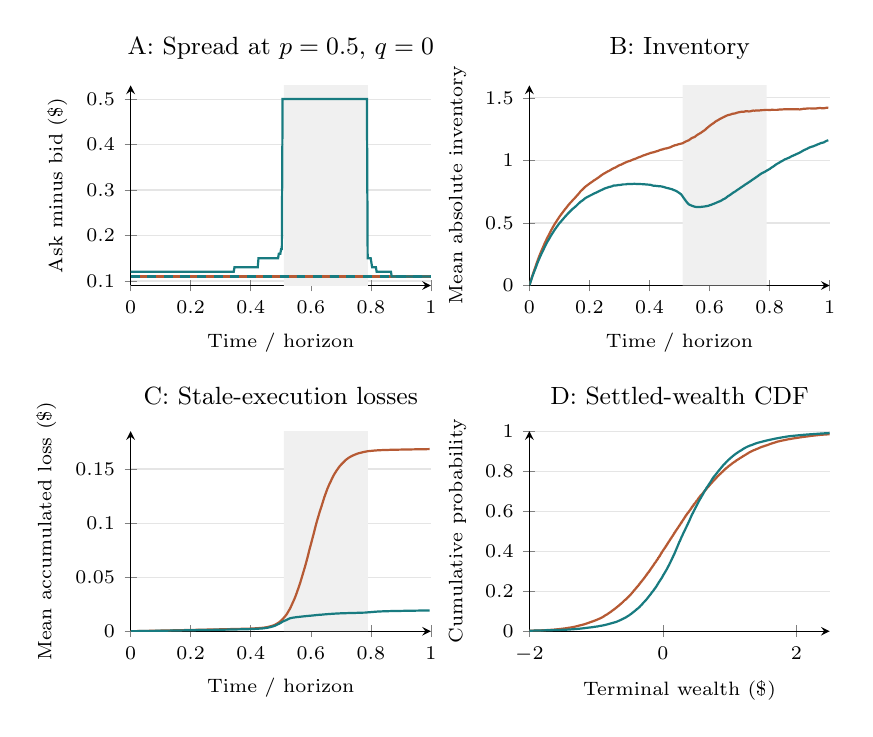
\begin{tikzpicture}
\begin{groupplot}[group style={group size=2 by 2,horizontal sep=1.25cm,vertical sep=1.85cm},
width=0.445\linewidth,height=0.34\linewidth,
label style={font=\scriptsize},tick label style={font=\scriptsize},
title style={font=\small},legend style={font=\tiny,draw=none,fill=none},
axis lines=left,ymajorgrids,grid style={gray!20},xmin=0,xmax=1,
cycle list name=color list]
\nextgroupplot[title={A: Spread at $p=0.5$, $q=0$},xlabel={Time / horizon},
ylabel={Ask minus bid (\$)},ymin=0.09,ymax=0.53,legend pos=south east]
\addplot[draw=none,fill=gray!12,forget plot] coordinates {(0.51,0) (0.79,0) (0.79,2) (0.51,2)} \closedcycle;
\addplot[thick,benchmark] coordinates {(0.00000,0.11000) (0.00250,0.11000) (0.00500,0.11000) (0.00750,0.11000) (0.01000,0.11000) (0.01250,0.11000) (0.01500,0.11000) (0.01750,0.11000) (0.02000,0.11000) (0.02250,0.11000) (0.02500,0.11000) (0.02750,0.11000) (0.03000,0.11000) (0.03250,0.11000) (0.03500,0.11000) (0.03750,0.11000) (0.04000,0.11000) (0.04250,0.11000) (0.04500,0.11000) (0.04750,0.11000) (0.05000,0.11000) (0.05250,0.11000) (0.05500,0.11000) (0.05750,0.11000) (0.06000,0.11000) (0.06250,0.11000) (0.06500,0.11000) (0.06750,0.11000) (0.07000,0.11000) (0.07250,0.11000) (0.07500,0.11000) (0.07750,0.11000) (0.08000,0.11000) (0.08250,0.11000) (0.08500,0.11000) (0.08750,0.11000) (0.09000,0.11000) (0.09250,0.11000) (0.09500,0.11000) (0.09750,0.11000) (0.10000,0.11000) (0.10250,0.11000) (0.10500,0.11000) (0.10750,0.11000) (0.11000,0.11000) (0.11275,0.11000) (0.11525,0.11000) (0.11775,0.11000) (0.12025,0.11000) (0.12275,0.11000) (0.12525,0.11000) (0.12775,0.11000) (0.13025,0.11000) (0.13275,0.11000) (0.13525,0.11000) (0.13775,0.11000) (0.14025,0.11000) (0.14275,0.11000) (0.14525,0.11000) (0.14775,0.11000) (0.15025,0.11000) (0.15275,0.11000) (0.15525,0.11000) (0.15775,0.11000) (0.16025,0.11000) (0.16275,0.11000) (0.16525,0.11000) (0.16775,0.11000) (0.17025,0.11000) (0.17275,0.11000) (0.17525,0.11000) (0.17775,0.11000) (0.18025,0.11000) (0.18275,0.11000) (0.18525,0.11000) (0.18775,0.11000) (0.19025,0.11000) (0.19275,0.11000) (0.19525,0.11000) (0.19775,0.11000) (0.20025,0.11000) (0.20275,0.11000) (0.20525,0.11000) (0.20775,0.11000) (0.21025,0.11000) (0.21275,0.11000) (0.21525,0.11000) (0.21775,0.11000) (0.22025,0.11000) (0.22300,0.11000) (0.22550,0.11000) (0.22800,0.11000) (0.23050,0.11000) (0.23300,0.11000) (0.23550,0.11000) (0.23800,0.11000) (0.24050,0.11000) (0.24300,0.11000) (0.24550,0.11000) (0.24800,0.11000) (0.25050,0.11000) (0.25300,0.11000) (0.25550,0.11000) (0.25800,0.11000) (0.26050,0.11000) (0.26300,0.11000) (0.26550,0.11000) (0.26800,0.11000) (0.27050,0.11000) (0.27300,0.11000) (0.27550,0.11000) (0.27800,0.11000) (0.28050,0.11000) (0.28300,0.11000) (0.28550,0.11000) (0.28800,0.11000) (0.29050,0.11000) (0.29300,0.11000) (0.29550,0.11000) (0.29800,0.11000) (0.30050,0.11000) (0.30300,0.11000) (0.30550,0.11000) (0.30800,0.11000) (0.31050,0.11000) (0.31300,0.11000) (0.31550,0.11000) (0.31800,0.11000) (0.32050,0.11000) (0.32300,0.11000) (0.32550,0.11000) (0.32800,0.11000) (0.33050,0.11000) (0.33325,0.11000) (0.33575,0.11000) (0.33825,0.11000) (0.34075,0.11000) (0.34325,0.11000) (0.34575,0.11000) (0.34825,0.11000) (0.35075,0.11000) (0.35325,0.11000) (0.35575,0.11000) (0.35825,0.11000) (0.36075,0.11000) (0.36325,0.11000) (0.36575,0.11000) (0.36825,0.11000) (0.37075,0.11000) (0.37325,0.11000) (0.37575,0.11000) (0.37825,0.11000) (0.38075,0.11000) (0.38325,0.11000) (0.38575,0.11000) (0.38825,0.11000) (0.39075,0.11000) (0.39325,0.11000) (0.39575,0.11000) (0.39825,0.11000) (0.40075,0.11000) (0.40325,0.11000) (0.40575,0.11000) (0.40825,0.11000) (0.41075,0.11000) (0.41325,0.11000) (0.41575,0.11000) (0.41825,0.11000) (0.42075,0.11000) (0.42325,0.11000) (0.42575,0.11000) (0.42825,0.11000) (0.43075,0.11000) (0.43325,0.11000) (0.43575,0.11000) (0.43825,0.11000) (0.44075,0.11000) (0.44325,0.11000) (0.44600,0.11000) (0.44850,0.11000) (0.45100,0.11000) (0.45350,0.11000) (0.45600,0.11000) (0.45850,0.11000) (0.46100,0.11000) (0.46350,0.11000) (0.46600,0.11000) (0.46850,0.11000) (0.47100,0.11000) (0.47350,0.11000) (0.47600,0.11000) (0.47850,0.11000) (0.48100,0.11000) (0.48350,0.11000) (0.48600,0.11000) (0.48850,0.11000) (0.49100,0.11000) (0.49350,0.11000) (0.49600,0.11000) (0.49850,0.11000) (0.50100,0.11000) (0.50350,0.11000) (0.50600,0.11000) (0.50850,0.11000) (0.51100,0.11000) (0.51350,0.11000) (0.51600,0.11000) (0.51850,0.11000) (0.52100,0.11000) (0.52350,0.11000) (0.52600,0.11000) (0.52850,0.11000) (0.53100,0.11000) (0.53350,0.11000) (0.53600,0.11000) (0.53850,0.11000) (0.54100,0.11000) (0.54350,0.11000) (0.54600,0.11000) (0.54850,0.11000) (0.55100,0.11000) (0.55350,0.11000) (0.55625,0.11000) (0.55875,0.11000) (0.56125,0.11000) (0.56375,0.11000) (0.56625,0.11000) (0.56875,0.11000) (0.57125,0.11000) (0.57375,0.11000) (0.57625,0.11000) (0.57875,0.11000) (0.58125,0.11000) (0.58375,0.11000) (0.58625,0.11000) (0.58875,0.11000) (0.59125,0.11000) (0.59375,0.11000) (0.59625,0.11000) (0.59875,0.11000) (0.60125,0.11000) (0.60375,0.11000) (0.60625,0.11000) (0.60875,0.11000) (0.61125,0.11000) (0.61375,0.11000) (0.61625,0.11000) (0.61875,0.11000) (0.62125,0.11000) (0.62375,0.11000) (0.62625,0.11000) (0.62875,0.11000) (0.63125,0.11000) (0.63375,0.11000) (0.63625,0.11000) (0.63875,0.11000) (0.64125,0.11000) (0.64375,0.11000) (0.64625,0.11000) (0.64875,0.11000) (0.65125,0.11000) (0.65375,0.11000) (0.65625,0.11000) (0.65875,0.11000) (0.66125,0.11000) (0.66375,0.11000) (0.66650,0.11000) (0.66900,0.11000) (0.67150,0.11000) (0.67400,0.11000) (0.67650,0.11000) (0.67900,0.11000) (0.68150,0.11000) (0.68400,0.11000) (0.68650,0.11000) (0.68900,0.11000) (0.69150,0.11000) (0.69400,0.11000) (0.69650,0.11000) (0.69900,0.11000) (0.70150,0.11000) (0.70400,0.11000) (0.70650,0.11000) (0.70900,0.11000) (0.71150,0.11000) (0.71400,0.11000) (0.71650,0.11000) (0.71900,0.11000) (0.72150,0.11000) (0.72400,0.11000) (0.72650,0.11000) (0.72900,0.11000) (0.73150,0.11000) (0.73400,0.11000) (0.73650,0.11000) (0.73900,0.11000) (0.74150,0.11000) (0.74400,0.11000) (0.74650,0.11000) (0.74900,0.11000) (0.75150,0.11000) (0.75400,0.11000) (0.75650,0.11000) (0.75900,0.11000) (0.76150,0.11000) (0.76400,0.11000) (0.76650,0.11000) (0.76900,0.11000) (0.77150,0.11000) (0.77400,0.11000) (0.77650,0.11000) (0.77925,0.11000) (0.78175,0.11000) (0.78425,0.11000) (0.78675,0.11000) (0.78925,0.11000) (0.79175,0.11000) (0.79425,0.11000) (0.79675,0.11000) (0.79925,0.11000) (0.80175,0.11000) (0.80425,0.11000) (0.80675,0.11000) (0.80925,0.11000) (0.81175,0.11000) (0.81425,0.11000) (0.81675,0.11000) (0.81925,0.11000) (0.82175,0.11000) (0.82425,0.11000) (0.82675,0.11000) (0.82925,0.11000) (0.83175,0.11000) (0.83425,0.11000) (0.83675,0.11000) (0.83925,0.11000) (0.84175,0.11000) (0.84425,0.11000) (0.84675,0.11000) (0.84925,0.11000) (0.85175,0.11000) (0.85425,0.11000) (0.85675,0.11000) (0.85925,0.11000) (0.86175,0.11000) (0.86425,0.11000) (0.86675,0.11000) (0.86925,0.11000) (0.87175,0.11000) (0.87425,0.11000) (0.87675,0.11000) (0.87925,0.11000) (0.88175,0.11000) (0.88425,0.11000) (0.88675,0.11000) (0.88950,0.11000) (0.89200,0.11000) (0.89450,0.11000) (0.89700,0.11000) (0.89950,0.11000) (0.90200,0.11000) (0.90450,0.11000) (0.90700,0.11000) (0.90950,0.11000) (0.91200,0.11000) (0.91450,0.11000) (0.91700,0.11000) (0.91950,0.11000) (0.92200,0.11000) (0.92450,0.11000) (0.92700,0.11000) (0.92950,0.11000) (0.93200,0.11000) (0.93450,0.11000) (0.93700,0.11000) (0.93950,0.11000) (0.94200,0.11000) (0.94450,0.11000) (0.94700,0.11000) (0.94950,0.11000) (0.95200,0.11000) (0.95450,0.11000) (0.95700,0.11000) (0.95950,0.11000) (0.96200,0.11000) (0.96450,0.11000) (0.96700,0.11000) (0.96950,0.11000) (0.97200,0.11000) (0.97450,0.11000) (0.97700,0.11000) (0.97950,0.11000) (0.98200,0.11000) (0.98450,0.11000) (0.98700,0.11000) (0.98950,0.11000) (0.99200,0.11000) (0.99450,0.11000) (0.99700,0.11000) (0.99975,0.11000)};

\addplot[thick,eventaware] coordinates {(0.00000,0.12000) (0.00250,0.12000) (0.00500,0.12000) (0.00750,0.12000) (0.01000,0.12000) (0.01250,0.12000) (0.01500,0.12000) (0.01750,0.12000) (0.02000,0.12000) (0.02250,0.12000) (0.02500,0.12000) (0.02750,0.12000) (0.03000,0.12000) (0.03250,0.12000) (0.03500,0.12000) (0.03750,0.12000) (0.04000,0.12000) (0.04250,0.12000) (0.04500,0.12000) (0.04750,0.12000) (0.05000,0.12000) (0.05250,0.12000) (0.05500,0.12000) (0.05750,0.12000) (0.06000,0.12000) (0.06250,0.12000) (0.06500,0.12000) (0.06750,0.12000) (0.07000,0.12000) (0.07250,0.12000) (0.07500,0.12000) (0.07750,0.12000) (0.08000,0.12000) (0.08250,0.12000) (0.08500,0.12000) (0.08750,0.12000) (0.09000,0.12000) (0.09250,0.12000) (0.09500,0.12000) (0.09750,0.12000) (0.10000,0.12000) (0.10250,0.12000) (0.10500,0.12000) (0.10750,0.12000) (0.11000,0.12000) (0.11275,0.12000) (0.11525,0.12000) (0.11775,0.12000) (0.12025,0.12000) (0.12275,0.12000) (0.12525,0.12000) (0.12775,0.12000) (0.13025,0.12000) (0.13275,0.12000) (0.13525,0.12000) (0.13775,0.12000) (0.14025,0.12000) (0.14275,0.12000) (0.14525,0.12000) (0.14775,0.12000) (0.15025,0.12000) (0.15275,0.12000) (0.15525,0.12000) (0.15775,0.12000) (0.16025,0.12000) (0.16275,0.12000) (0.16525,0.12000) (0.16775,0.12000) (0.17025,0.12000) (0.17275,0.12000) (0.17525,0.12000) (0.17775,0.12000) (0.18025,0.12000) (0.18275,0.12000) (0.18525,0.12000) (0.18775,0.12000) (0.19025,0.12000) (0.19275,0.12000) (0.19525,0.12000) (0.19775,0.12000) (0.20025,0.12000) (0.20275,0.12000) (0.20525,0.12000) (0.20775,0.12000) (0.21025,0.12000) (0.21275,0.12000) (0.21525,0.12000) (0.21775,0.12000) (0.22025,0.12000) (0.22300,0.12000) (0.22550,0.12000) (0.22800,0.12000) (0.23050,0.12000) (0.23300,0.12000) (0.23550,0.12000) (0.23800,0.12000) (0.24050,0.12000) (0.24300,0.12000) (0.24550,0.12000) (0.24800,0.12000) (0.25050,0.12000) (0.25300,0.12000) (0.25550,0.12000) (0.25800,0.12000) (0.26050,0.12000) (0.26300,0.12000) (0.26550,0.12000) (0.26800,0.12000) (0.27050,0.12000) (0.27300,0.12000) (0.27550,0.12000) (0.27800,0.12000) (0.28050,0.12000) (0.28300,0.12000) (0.28550,0.12000) (0.28800,0.12000) (0.29050,0.12000) (0.29300,0.12000) (0.29550,0.12000) (0.29800,0.12000) (0.30050,0.12000) (0.30300,0.12000) (0.30550,0.12000) (0.30800,0.12000) (0.31050,0.12000) (0.31300,0.12000) (0.31550,0.12000) (0.31800,0.12000) (0.32050,0.12000) (0.32300,0.12000) (0.32550,0.12000) (0.32800,0.12000) (0.33050,0.12000) (0.33325,0.12000) (0.33575,0.12000) (0.33825,0.12000) (0.34075,0.12000) (0.34325,0.12000) (0.34575,0.13000) (0.34825,0.13000) (0.35075,0.13000) (0.35325,0.13000) (0.35575,0.13000) (0.35825,0.13000) (0.36075,0.13000) (0.36325,0.13000) (0.36575,0.13000) (0.36825,0.13000) (0.37075,0.13000) (0.37325,0.13000) (0.37575,0.13000) (0.37825,0.13000) (0.38075,0.13000) (0.38325,0.13000) (0.38575,0.13000) (0.38825,0.13000) (0.39075,0.13000) (0.39325,0.13000) (0.39575,0.13000) (0.39825,0.13000) (0.40075,0.13000) (0.40325,0.13000) (0.40575,0.13000) (0.40825,0.13000) (0.41075,0.13000) (0.41325,0.13000) (0.41575,0.13000) (0.41825,0.13000) (0.42075,0.13000) (0.42325,0.13000) (0.42575,0.15000) (0.42825,0.15000) (0.43075,0.15000) (0.43325,0.15000) (0.43575,0.15000) (0.43825,0.15000) (0.44075,0.15000) (0.44325,0.15000) (0.44600,0.15000) (0.44850,0.15000) (0.45100,0.15000) (0.45350,0.15000) (0.45600,0.15000) (0.45850,0.15000) (0.46100,0.15000) (0.46350,0.15000) (0.46600,0.15000) (0.46850,0.15000) (0.47100,0.15000) (0.47350,0.15000) (0.47600,0.15000) (0.47850,0.15000) (0.48100,0.15000) (0.48350,0.15000) (0.48600,0.15000) (0.48850,0.15000) (0.49100,0.15000) (0.49350,0.16000) (0.49600,0.16000) (0.49850,0.16000) (0.50100,0.17000) (0.50350,0.17000) (0.50600,0.50000) (0.50850,0.50000) (0.51100,0.50000) (0.51350,0.50000) (0.51600,0.50000) (0.51850,0.50000) (0.52100,0.50000) (0.52350,0.50000) (0.52600,0.50000) (0.52850,0.50000) (0.53100,0.50000) (0.53350,0.50000) (0.53600,0.50000) (0.53850,0.50000) (0.54100,0.50000) (0.54350,0.50000) (0.54600,0.50000) (0.54850,0.50000) (0.55100,0.50000) (0.55350,0.50000) (0.55625,0.50000) (0.55875,0.50000) (0.56125,0.50000) (0.56375,0.50000) (0.56625,0.50000) (0.56875,0.50000) (0.57125,0.50000) (0.57375,0.50000) (0.57625,0.50000) (0.57875,0.50000) (0.58125,0.50000) (0.58375,0.50000) (0.58625,0.50000) (0.58875,0.50000) (0.59125,0.50000) (0.59375,0.50000) (0.59625,0.50000) (0.59875,0.50000) (0.60125,0.50000) (0.60375,0.50000) (0.60625,0.50000) (0.60875,0.50000) (0.61125,0.50000) (0.61375,0.50000) (0.61625,0.50000) (0.61875,0.50000) (0.62125,0.50000) (0.62375,0.50000) (0.62625,0.50000) (0.62875,0.50000) (0.63125,0.50000) (0.63375,0.50000) (0.63625,0.50000) (0.63875,0.50000) (0.64125,0.50000) (0.64375,0.50000) (0.64625,0.50000) (0.64875,0.50000) (0.65125,0.50000) (0.65375,0.50000) (0.65625,0.50000) (0.65875,0.50000) (0.66125,0.50000) (0.66375,0.50000) (0.66650,0.50000) (0.66900,0.50000) (0.67150,0.50000) (0.67400,0.50000) (0.67650,0.50000) (0.67900,0.50000) (0.68150,0.50000) (0.68400,0.50000) (0.68650,0.50000) (0.68900,0.50000) (0.69150,0.50000) (0.69400,0.50000) (0.69650,0.50000) (0.69900,0.50000) (0.70150,0.50000) (0.70400,0.50000) (0.70650,0.50000) (0.70900,0.50000) (0.71150,0.50000) (0.71400,0.50000) (0.71650,0.50000) (0.71900,0.50000) (0.72150,0.50000) (0.72400,0.50000) (0.72650,0.50000) (0.72900,0.50000) (0.73150,0.50000) (0.73400,0.50000) (0.73650,0.50000) (0.73900,0.50000) (0.74150,0.50000) (0.74400,0.50000) (0.74650,0.50000) (0.74900,0.50000) (0.75150,0.50000) (0.75400,0.50000) (0.75650,0.50000) (0.75900,0.50000) (0.76150,0.50000) (0.76400,0.50000) (0.76650,0.50000) (0.76900,0.50000) (0.77150,0.50000) (0.77400,0.50000) (0.77650,0.50000) (0.77925,0.50000) (0.78175,0.50000) (0.78425,0.50000) (0.78675,0.50000) (0.78925,0.15000) (0.79175,0.15000) (0.79425,0.15000) (0.79675,0.15000) (0.79925,0.15000) (0.80175,0.14000) (0.80425,0.13000) (0.80675,0.13000) (0.80925,0.13000) (0.81175,0.13000) (0.81425,0.13000) (0.81675,0.13000) (0.81925,0.12000) (0.82175,0.12000) (0.82425,0.12000) (0.82675,0.12000) (0.82925,0.12000) (0.83175,0.12000) (0.83425,0.12000) (0.83675,0.12000) (0.83925,0.12000) (0.84175,0.12000) (0.84425,0.12000) (0.84675,0.12000) (0.84925,0.12000) (0.85175,0.12000) (0.85425,0.12000) (0.85675,0.12000) (0.85925,0.12000) (0.86175,0.12000) (0.86425,0.12000) (0.86675,0.12000) (0.86925,0.11000) (0.87175,0.11000) (0.87425,0.11000) (0.87675,0.11000) (0.87925,0.11000) (0.88175,0.11000) (0.88425,0.11000) (0.88675,0.11000) (0.88950,0.11000) (0.89200,0.11000) (0.89450,0.11000) (0.89700,0.11000) (0.89950,0.11000) (0.90200,0.11000) (0.90450,0.11000) (0.90700,0.11000) (0.90950,0.11000) (0.91200,0.11000) (0.91450,0.11000) (0.91700,0.11000) (0.91950,0.11000) (0.92200,0.11000) (0.92450,0.11000) (0.92700,0.11000) (0.92950,0.11000) (0.93200,0.11000) (0.93450,0.11000) (0.93700,0.11000) (0.93950,0.11000) (0.94200,0.11000) (0.94450,0.11000) (0.94700,0.11000) (0.94950,0.11000) (0.95200,0.11000) (0.95450,0.11000) (0.95700,0.11000) (0.95950,0.11000) (0.96200,0.11000) (0.96450,0.11000) (0.96700,0.11000) (0.96950,0.11000) (0.97200,0.11000) (0.97450,0.11000) (0.97700,0.11000) (0.97950,0.11000) (0.98200,0.11000) (0.98450,0.11000) (0.98700,0.11000) (0.98950,0.11000) (0.99200,0.11000) (0.99450,0.11000) (0.99700,0.11000) (0.99975,0.11000)};

\addplot[thick,eventaware,dashed] coordinates {(0.00000,0.11000) (0.00250,0.11000) (0.00500,0.11000) (0.00750,0.11000) (0.01000,0.11000) (0.01250,0.11000) (0.01500,0.11000) (0.01750,0.11000) (0.02000,0.11000) (0.02250,0.11000) (0.02500,0.11000) (0.02750,0.11000) (0.03000,0.11000) (0.03250,0.11000) (0.03500,0.11000) (0.03750,0.11000) (0.04000,0.11000) (0.04250,0.11000) (0.04500,0.11000) (0.04750,0.11000) (0.05000,0.11000) (0.05250,0.11000) (0.05500,0.11000) (0.05750,0.11000) (0.06000,0.11000) (0.06250,0.11000) (0.06500,0.11000) (0.06750,0.11000) (0.07000,0.11000) (0.07250,0.11000) (0.07500,0.11000) (0.07750,0.11000) (0.08000,0.11000) (0.08250,0.11000) (0.08500,0.11000) (0.08750,0.11000) (0.09000,0.11000) (0.09250,0.11000) (0.09500,0.11000) (0.09750,0.11000) (0.10000,0.11000) (0.10250,0.11000) (0.10500,0.11000) (0.10750,0.11000) (0.11000,0.11000) (0.11275,0.11000) (0.11525,0.11000) (0.11775,0.11000) (0.12025,0.11000) (0.12275,0.11000) (0.12525,0.11000) (0.12775,0.11000) (0.13025,0.11000) (0.13275,0.11000) (0.13525,0.11000) (0.13775,0.11000) (0.14025,0.11000) (0.14275,0.11000) (0.14525,0.11000) (0.14775,0.11000) (0.15025,0.11000) (0.15275,0.11000) (0.15525,0.11000) (0.15775,0.11000) (0.16025,0.11000) (0.16275,0.11000) (0.16525,0.11000) (0.16775,0.11000) (0.17025,0.11000) (0.17275,0.11000) (0.17525,0.11000) (0.17775,0.11000) (0.18025,0.11000) (0.18275,0.11000) (0.18525,0.11000) (0.18775,0.11000) (0.19025,0.11000) (0.19275,0.11000) (0.19525,0.11000) (0.19775,0.11000) (0.20025,0.11000) (0.20275,0.11000) (0.20525,0.11000) (0.20775,0.11000) (0.21025,0.11000) (0.21275,0.11000) (0.21525,0.11000) (0.21775,0.11000) (0.22025,0.11000) (0.22300,0.11000) (0.22550,0.11000) (0.22800,0.11000) (0.23050,0.11000) (0.23300,0.11000) (0.23550,0.11000) (0.23800,0.11000) (0.24050,0.11000) (0.24300,0.11000) (0.24550,0.11000) (0.24800,0.11000) (0.25050,0.11000) (0.25300,0.11000) (0.25550,0.11000) (0.25800,0.11000) (0.26050,0.11000) (0.26300,0.11000) (0.26550,0.11000) (0.26800,0.11000) (0.27050,0.11000) (0.27300,0.11000) (0.27550,0.11000) (0.27800,0.11000) (0.28050,0.11000) (0.28300,0.11000) (0.28550,0.11000) (0.28800,0.11000) (0.29050,0.11000) (0.29300,0.11000) (0.29550,0.11000) (0.29800,0.11000) (0.30050,0.11000) (0.30300,0.11000) (0.30550,0.11000) (0.30800,0.11000) (0.31050,0.11000) (0.31300,0.11000) (0.31550,0.11000) (0.31800,0.11000) (0.32050,0.11000) (0.32300,0.11000) (0.32550,0.11000) (0.32800,0.11000) (0.33050,0.11000) (0.33325,0.11000) (0.33575,0.11000) (0.33825,0.11000) (0.34075,0.11000) (0.34325,0.11000) (0.34575,0.11000) (0.34825,0.11000) (0.35075,0.11000) (0.35325,0.11000) (0.35575,0.11000) (0.35825,0.11000) (0.36075,0.11000) (0.36325,0.11000) (0.36575,0.11000) (0.36825,0.11000) (0.37075,0.11000) (0.37325,0.11000) (0.37575,0.11000) (0.37825,0.11000) (0.38075,0.11000) (0.38325,0.11000) (0.38575,0.11000) (0.38825,0.11000) (0.39075,0.11000) (0.39325,0.11000) (0.39575,0.11000) (0.39825,0.11000) (0.40075,0.11000) (0.40325,0.11000) (0.40575,0.11000) (0.40825,0.11000) (0.41075,0.11000) (0.41325,0.11000) (0.41575,0.11000) (0.41825,0.11000) (0.42075,0.11000) (0.42325,0.11000) (0.42575,0.11000) (0.42825,0.11000) (0.43075,0.11000) (0.43325,0.11000) (0.43575,0.11000) (0.43825,0.11000) (0.44075,0.11000) (0.44325,0.11000) (0.44600,0.11000) (0.44850,0.11000) (0.45100,0.11000) (0.45350,0.11000) (0.45600,0.11000) (0.45850,0.11000) (0.46100,0.11000) (0.46350,0.11000) (0.46600,0.11000) (0.46850,0.11000) (0.47100,0.11000) (0.47350,0.11000) (0.47600,0.11000) (0.47850,0.11000) (0.48100,0.11000) (0.48350,0.11000) (0.48600,0.11000) (0.48850,0.11000) (0.49100,0.11000) (0.49350,0.11000) (0.49600,0.11000) (0.49850,0.11000) (0.50100,0.11000) (0.50350,0.11000) (0.50600,0.11000) (0.50850,0.11000) (0.51100,0.11000) (0.51350,0.11000) (0.51600,0.11000) (0.51850,0.11000) (0.52100,0.11000) (0.52350,0.11000) (0.52600,0.11000) (0.52850,0.11000) (0.53100,0.11000) (0.53350,0.11000) (0.53600,0.11000) (0.53850,0.11000) (0.54100,0.11000) (0.54350,0.11000) (0.54600,0.11000) (0.54850,0.11000) (0.55100,0.11000) (0.55350,0.11000) (0.55625,0.11000) (0.55875,0.11000) (0.56125,0.11000) (0.56375,0.11000) (0.56625,0.11000) (0.56875,0.11000) (0.57125,0.11000) (0.57375,0.11000) (0.57625,0.11000) (0.57875,0.11000) (0.58125,0.11000) (0.58375,0.11000) (0.58625,0.11000) (0.58875,0.11000) (0.59125,0.11000) (0.59375,0.11000) (0.59625,0.11000) (0.59875,0.11000) (0.60125,0.11000) (0.60375,0.11000) (0.60625,0.11000) (0.60875,0.11000) (0.61125,0.11000) (0.61375,0.11000) (0.61625,0.11000) (0.61875,0.11000) (0.62125,0.11000) (0.62375,0.11000) (0.62625,0.11000) (0.62875,0.11000) (0.63125,0.11000) (0.63375,0.11000) (0.63625,0.11000) (0.63875,0.11000) (0.64125,0.11000) (0.64375,0.11000) (0.64625,0.11000) (0.64875,0.11000) (0.65125,0.11000) (0.65375,0.11000) (0.65625,0.11000) (0.65875,0.11000) (0.66125,0.11000) (0.66375,0.11000) (0.66650,0.11000) (0.66900,0.11000) (0.67150,0.11000) (0.67400,0.11000) (0.67650,0.11000) (0.67900,0.11000) (0.68150,0.11000) (0.68400,0.11000) (0.68650,0.11000) (0.68900,0.11000) (0.69150,0.11000) (0.69400,0.11000) (0.69650,0.11000) (0.69900,0.11000) (0.70150,0.11000) (0.70400,0.11000) (0.70650,0.11000) (0.70900,0.11000) (0.71150,0.11000) (0.71400,0.11000) (0.71650,0.11000) (0.71900,0.11000) (0.72150,0.11000) (0.72400,0.11000) (0.72650,0.11000) (0.72900,0.11000) (0.73150,0.11000) (0.73400,0.11000) (0.73650,0.11000) (0.73900,0.11000) (0.74150,0.11000) (0.74400,0.11000) (0.74650,0.11000) (0.74900,0.11000) (0.75150,0.11000) (0.75400,0.11000) (0.75650,0.11000) (0.75900,0.11000) (0.76150,0.11000) (0.76400,0.11000) (0.76650,0.11000) (0.76900,0.11000) (0.77150,0.11000) (0.77400,0.11000) (0.77650,0.11000) (0.77925,0.11000) (0.78175,0.11000) (0.78425,0.11000) (0.78675,0.11000) (0.78925,0.11000) (0.79175,0.11000) (0.79425,0.11000) (0.79675,0.11000) (0.79925,0.11000) (0.80175,0.11000) (0.80425,0.11000) (0.80675,0.11000) (0.80925,0.11000) (0.81175,0.11000) (0.81425,0.11000) (0.81675,0.11000) (0.81925,0.11000) (0.82175,0.11000) (0.82425,0.11000) (0.82675,0.11000) (0.82925,0.11000) (0.83175,0.11000) (0.83425,0.11000) (0.83675,0.11000) (0.83925,0.11000) (0.84175,0.11000) (0.84425,0.11000) (0.84675,0.11000) (0.84925,0.11000) (0.85175,0.11000) (0.85425,0.11000) (0.85675,0.11000) (0.85925,0.11000) (0.86175,0.11000) (0.86425,0.11000) (0.86675,0.11000) (0.86925,0.11000) (0.87175,0.11000) (0.87425,0.11000) (0.87675,0.11000) (0.87925,0.11000) (0.88175,0.11000) (0.88425,0.11000) (0.88675,0.11000) (0.88950,0.11000) (0.89200,0.11000) (0.89450,0.11000) (0.89700,0.11000) (0.89950,0.11000) (0.90200,0.11000) (0.90450,0.11000) (0.90700,0.11000) (0.90950,0.11000) (0.91200,0.11000) (0.91450,0.11000) (0.91700,0.11000) (0.91950,0.11000) (0.92200,0.11000) (0.92450,0.11000) (0.92700,0.11000) (0.92950,0.11000) (0.93200,0.11000) (0.93450,0.11000) (0.93700,0.11000) (0.93950,0.11000) (0.94200,0.11000) (0.94450,0.11000) (0.94700,0.11000) (0.94950,0.11000) (0.95200,0.11000) (0.95450,0.11000) (0.95700,0.11000) (0.95950,0.11000) (0.96200,0.11000) (0.96450,0.11000) (0.96700,0.11000) (0.96950,0.11000) (0.97200,0.11000) (0.97450,0.11000) (0.97700,0.11000) (0.97950,0.11000) (0.98200,0.11000) (0.98450,0.11000) (0.98700,0.11000) (0.98950,0.11000) (0.99200,0.11000) (0.99450,0.11000) (0.99700,0.11000) (0.99975,0.11000)};

\nextgroupplot[title={B: Inventory},xlabel={Time / horizon},
ylabel={Mean absolute inventory},ymin=0,ymax=1.6]
\addplot[draw=none,fill=gray!12,forget plot] coordinates {(0.51,0) (0.79,0) (0.79,2) (0.51,2)} \closedcycle;
\addplot[thick,benchmark] coordinates {(0.00025,0.00213) (0.00525,0.04170) (0.01025,0.08090) (0.01525,0.11613) (0.02025,0.14950) (0.02525,0.18547) (0.03025,0.21833) (0.03525,0.24897) (0.04025,0.27810) (0.04525,0.30530) (0.05025,0.33360) (0.05525,0.35920) (0.06025,0.38490) (0.06525,0.40573) (0.07025,0.43117) (0.07525,0.45323) (0.08025,0.47503) (0.08525,0.49540) (0.09025,0.51360) (0.09525,0.53213) (0.10025,0.55073) (0.10525,0.56693) (0.11025,0.58267) (0.11525,0.59897) (0.12025,0.61413) (0.12525,0.62860) (0.13025,0.64440) (0.13525,0.65820) (0.14025,0.67093) (0.14525,0.68473) (0.15025,0.69627) (0.15525,0.71030) (0.16025,0.72360) (0.16525,0.73690) (0.17025,0.75293) (0.17525,0.76410) (0.18025,0.77583) (0.18525,0.78790) (0.19025,0.79710) (0.19525,0.80590) (0.20025,0.81523) (0.20525,0.82340) (0.21025,0.83140) (0.21525,0.84090) (0.22025,0.84777) (0.22525,0.85600) (0.23025,0.86420) (0.23525,0.87343) (0.24025,0.88220) (0.24525,0.89057) (0.25025,0.89757) (0.25525,0.90397) (0.26025,0.91127) (0.26525,0.91680) (0.27025,0.92333) (0.27525,0.93127) (0.28025,0.93780) (0.28525,0.94197) (0.29025,0.94913) (0.29525,0.95610) (0.30025,0.96253) (0.30525,0.96633) (0.31025,0.97213) (0.31525,0.97817) (0.32025,0.98383) (0.32525,0.98900) (0.33025,0.99380) (0.33525,0.99673) (0.34025,1.00200) (0.34525,1.00733) (0.35025,1.01123) (0.35525,1.01577) (0.36025,1.02147) (0.36525,1.02620) (0.37025,1.02993) (0.37525,1.03560) (0.38025,1.04063) (0.38525,1.04410) (0.39025,1.04910) (0.39525,1.05280) (0.40025,1.05713) (0.40525,1.06147) (0.41025,1.06367) (0.41525,1.06683) (0.42025,1.07067) (0.42525,1.07440) (0.43025,1.07840) (0.43525,1.08367) (0.44025,1.08683) (0.44525,1.08977) (0.45025,1.09413) (0.45525,1.09590) (0.46025,1.09867) (0.46525,1.10253) (0.47025,1.10620) (0.47525,1.11237) (0.48025,1.11763) (0.48525,1.12197) (0.49025,1.12393) (0.49525,1.12870) (0.50025,1.13143) (0.50525,1.13443) (0.51025,1.13747) (0.51525,1.14450) (0.52025,1.15110) (0.52525,1.15597) (0.53025,1.16087) (0.53525,1.16913) (0.54025,1.17833) (0.54525,1.18367) (0.55025,1.18750) (0.55525,1.19763) (0.56025,1.20630) (0.56525,1.21297) (0.57025,1.21963) (0.57525,1.22893) (0.58025,1.23647) (0.58525,1.24497) (0.59025,1.25707) (0.59525,1.26657) (0.60025,1.27657) (0.60525,1.28583) (0.61025,1.29367) (0.61525,1.30233) (0.62025,1.31210) (0.62525,1.31850) (0.63025,1.32537) (0.63525,1.33303) (0.64025,1.33887) (0.64525,1.34510) (0.65025,1.35070) (0.65525,1.35697) (0.66025,1.36150) (0.66525,1.36473) (0.67025,1.36733) (0.67525,1.37293) (0.68025,1.37457) (0.68525,1.37640) (0.69025,1.38083) (0.69525,1.38417) (0.70025,1.38640) (0.70525,1.38883) (0.71025,1.38977) (0.71525,1.39027) (0.72025,1.39333) (0.72525,1.39353) (0.73025,1.39197) (0.73525,1.39270) (0.74025,1.39640) (0.74525,1.39877) (0.75025,1.39800) (0.75525,1.40000) (0.76025,1.39990) (0.76525,1.39983) (0.77025,1.40097) (0.77525,1.40237) (0.78025,1.40250) (0.78525,1.40420) (0.79025,1.40453) (0.79525,1.40413) (0.80025,1.40347) (0.80525,1.40460) (0.81025,1.40467) (0.81525,1.40443) (0.82025,1.40437) (0.82525,1.40460) (0.83025,1.40650) (0.83525,1.40733) (0.84025,1.40817) (0.84525,1.40837) (0.85025,1.41033) (0.85525,1.40917) (0.86025,1.41000) (0.86525,1.40853) (0.87025,1.40977) (0.87525,1.41010) (0.88025,1.40993) (0.88525,1.40960) (0.89025,1.40940) (0.89525,1.40883) (0.90025,1.40803) (0.90525,1.41007) (0.91025,1.41213) (0.91525,1.41347) (0.92025,1.41410) (0.92525,1.41533) (0.93025,1.41643) (0.93525,1.41643) (0.94025,1.41537) (0.94525,1.41470) (0.95025,1.41543) (0.95525,1.41600) (0.96025,1.41800) (0.96525,1.41893) (0.97025,1.41860) (0.97525,1.41760) (0.98025,1.41670) (0.98525,1.41983) (0.99025,1.42160) (0.99525,1.42057)};
\addplot[thick,eventaware] coordinates {(0.00025,0.00193) (0.00525,0.03787) (0.01025,0.07377) (0.01525,0.10603) (0.02025,0.13603) (0.02525,0.16940) (0.03025,0.19943) (0.03525,0.22727) (0.04025,0.25357) (0.04525,0.27757) (0.05025,0.30357) (0.05525,0.32777) (0.06025,0.35143) (0.06525,0.36997) (0.07025,0.39257) (0.07525,0.41170) (0.08025,0.43053) (0.08525,0.44927) (0.09025,0.46570) (0.09525,0.48233) (0.10025,0.49863) (0.10525,0.51183) (0.11025,0.52577) (0.11525,0.54020) (0.12025,0.55373) (0.12525,0.56680) (0.13025,0.58003) (0.13525,0.59167) (0.14025,0.60367) (0.14525,0.61513) (0.15025,0.62467) (0.15525,0.63517) (0.16025,0.64677) (0.16525,0.65837) (0.17025,0.66967) (0.17525,0.67713) (0.18025,0.68640) (0.18525,0.69700) (0.19025,0.70420) (0.19525,0.71070) (0.20025,0.71667) (0.20525,0.72287) (0.21025,0.72890) (0.21525,0.73563) (0.22025,0.74070) (0.22525,0.74610) (0.23025,0.75230) (0.23525,0.75860) (0.24025,0.76350) (0.24525,0.76967) (0.25025,0.77520) (0.25525,0.77913) (0.26025,0.78357) (0.26525,0.78783) (0.27025,0.79037) (0.27525,0.79363) (0.28025,0.79893) (0.28525,0.79910) (0.29025,0.80070) (0.29525,0.80313) (0.30025,0.80403) (0.30525,0.80517) (0.31025,0.80810) (0.31525,0.80880) (0.32025,0.80863) (0.32525,0.81107) (0.33025,0.81163) (0.33525,0.81107) (0.34025,0.81177) (0.34525,0.81257) (0.35025,0.81310) (0.35525,0.81220) (0.36025,0.81190) (0.36525,0.81143) (0.37025,0.81087) (0.37525,0.81063) (0.38025,0.80963) (0.38525,0.80887) (0.39025,0.80760) (0.39525,0.80667) (0.40025,0.80627) (0.40525,0.80403) (0.41025,0.79927) (0.41525,0.79743) (0.42025,0.79700) (0.42525,0.79553) (0.43025,0.79427) (0.43525,0.79360) (0.44025,0.79210) (0.44525,0.78897) (0.45025,0.78587) (0.45525,0.78147) (0.46025,0.77880) (0.46525,0.77603) (0.47025,0.77277) (0.47525,0.76943) (0.48025,0.76393) (0.48525,0.75940) (0.49025,0.75427) (0.49525,0.74580) (0.50025,0.73797) (0.50525,0.72900) (0.51025,0.71243) (0.51525,0.69513) (0.52025,0.67883) (0.52525,0.66307) (0.53025,0.65010) (0.53525,0.64383) (0.54025,0.63873) (0.54525,0.63417) (0.55025,0.63017) (0.55525,0.62803) (0.56025,0.62703) (0.56525,0.62707) (0.57025,0.62810) (0.57525,0.62997) (0.58025,0.63093) (0.58525,0.63260) (0.59025,0.63500) (0.59525,0.63707) (0.60025,0.64163) (0.60525,0.64513) (0.61025,0.65030) (0.61525,0.65470) (0.62025,0.65943) (0.62525,0.66540) (0.63025,0.67007) (0.63525,0.67493) (0.64025,0.68073) (0.64525,0.68870) (0.65025,0.69420) (0.65525,0.70220) (0.66025,0.71240) (0.66525,0.71943) (0.67025,0.72747) (0.67525,0.73673) (0.68025,0.74480) (0.68525,0.75173) (0.69025,0.76073) (0.69525,0.76870) (0.70025,0.77663) (0.70525,0.78523) (0.71025,0.79270) (0.71525,0.80140) (0.72025,0.80947) (0.72525,0.81693) (0.73025,0.82510) (0.73525,0.83310) (0.74025,0.84153) (0.74525,0.84953) (0.75025,0.85760) (0.75525,0.86633) (0.76025,0.87420) (0.76525,0.88393) (0.77025,0.89210) (0.77525,0.89927) (0.78025,0.90523) (0.78525,0.91113) (0.79025,0.91867) (0.79525,0.92537) (0.80025,0.93183) (0.80525,0.94157) (0.81025,0.94863) (0.81525,0.95677) (0.82025,0.96613) (0.82525,0.97350) (0.83025,0.97987) (0.83525,0.98747) (0.84025,0.99413) (0.84525,1.00060) (0.85025,1.00857) (0.85525,1.01277) (0.86025,1.01793) (0.86525,1.02280) (0.87025,1.02967) (0.87525,1.03573) (0.88025,1.04097) (0.88525,1.04593) (0.89025,1.05190) (0.89525,1.05700) (0.90025,1.06253) (0.90525,1.06960) (0.91025,1.07703) (0.91525,1.08367) (0.92025,1.08867) (0.92525,1.09430) (0.93025,1.10100) (0.93525,1.10597) (0.94025,1.10980) (0.94525,1.11340) (0.95025,1.11840) (0.95525,1.12307) (0.96025,1.12883) (0.96525,1.13297) (0.97025,1.13870) (0.97525,1.14143) (0.98025,1.14443) (0.98525,1.15167) (0.99025,1.15773) (0.99525,1.16147)};
\nextgroupplot[title={C: Stale-execution losses},xlabel={Time / horizon},
ylabel={Mean accumulated loss (\$)},ymin=0,ymax=0.185,
yticklabel style={/pgf/number format/fixed,/pgf/number format/precision=2}]
\addplot[draw=none,fill=gray!12,forget plot] coordinates {(0.51,0) (0.79,0) (0.79,2) (0.51,2)} \closedcycle;
\addplot[thick,benchmark] coordinates {(0.00025,0.00000) (0.00525,0.00002) (0.01025,0.00006) (0.01525,0.00009) (0.02025,0.00012) (0.02525,0.00015) (0.03025,0.00019) (0.03525,0.00021) (0.04025,0.00023) (0.04525,0.00026) (0.05025,0.00029) (0.05525,0.00032) (0.06025,0.00035) (0.06525,0.00038) (0.07025,0.00040) (0.07525,0.00044) (0.08025,0.00046) (0.08525,0.00049) (0.09025,0.00053) (0.09525,0.00056) (0.10025,0.00059) (0.10525,0.00061) (0.11025,0.00064) (0.11525,0.00067) (0.12025,0.00070) (0.12525,0.00073) (0.13025,0.00075) (0.13525,0.00079) (0.14025,0.00082) (0.14525,0.00085) (0.15025,0.00089) (0.15525,0.00091) (0.16025,0.00095) (0.16525,0.00098) (0.17025,0.00101) (0.17525,0.00104) (0.18025,0.00106) (0.18525,0.00109) (0.19025,0.00112) (0.19525,0.00115) (0.20025,0.00118) (0.20525,0.00122) (0.21025,0.00124) (0.21525,0.00127) (0.22025,0.00131) (0.22525,0.00134) (0.23025,0.00138) (0.23525,0.00140) (0.24025,0.00144) (0.24525,0.00147) (0.25025,0.00150) (0.25525,0.00152) (0.26025,0.00156) (0.26525,0.00158) (0.27025,0.00160) (0.27525,0.00163) (0.28025,0.00165) (0.28525,0.00168) (0.29025,0.00172) (0.29525,0.00175) (0.30025,0.00178) (0.30525,0.00181) (0.31025,0.00184) (0.31525,0.00186) (0.32025,0.00190) (0.32525,0.00192) (0.33025,0.00196) (0.33525,0.00200) (0.34025,0.00204) (0.34525,0.00207) (0.35025,0.00209) (0.35525,0.00213) (0.36025,0.00216) (0.36525,0.00219) (0.37025,0.00223) (0.37525,0.00226) (0.38025,0.00229) (0.38525,0.00235) (0.39025,0.00238) (0.39525,0.00242) (0.40025,0.00247) (0.40525,0.00254) (0.41025,0.00260) (0.41525,0.00269) (0.42025,0.00278) (0.42525,0.00288) (0.43025,0.00299) (0.43525,0.00309) (0.44025,0.00321) (0.44525,0.00338) (0.45025,0.00361) (0.45525,0.00385) (0.46025,0.00421) (0.46525,0.00450) (0.47025,0.00495) (0.47525,0.00540) (0.48025,0.00593) (0.48525,0.00668) (0.49025,0.00752) (0.49525,0.00847) (0.50025,0.00960) (0.50525,0.01099) (0.51025,0.01246) (0.51525,0.01413) (0.52025,0.01593) (0.52525,0.01835) (0.53025,0.02069) (0.53525,0.02360) (0.54025,0.02672) (0.54525,0.02978) (0.55025,0.03325) (0.55525,0.03718) (0.56025,0.04113) (0.56525,0.04539) (0.57025,0.05001) (0.57525,0.05473) (0.58025,0.05934) (0.58525,0.06435) (0.59025,0.06961) (0.59525,0.07531) (0.60025,0.08037) (0.60525,0.08573) (0.61025,0.09090) (0.61525,0.09651) (0.62025,0.10173) (0.62525,0.10636) (0.63025,0.11116) (0.63525,0.11522) (0.64025,0.11970) (0.64525,0.12418) (0.65025,0.12799) (0.65525,0.13180) (0.66025,0.13507) (0.66525,0.13798) (0.67025,0.14093) (0.67525,0.14378) (0.68025,0.14615) (0.68525,0.14832) (0.69025,0.15035) (0.69525,0.15227) (0.70025,0.15384) (0.70525,0.15534) (0.71025,0.15666) (0.71525,0.15813) (0.72025,0.15919) (0.72525,0.16025) (0.73025,0.16108) (0.73525,0.16185) (0.74025,0.16255) (0.74525,0.16312) (0.75025,0.16368) (0.75525,0.16425) (0.76025,0.16467) (0.76525,0.16498) (0.77025,0.16532) (0.77525,0.16571) (0.78025,0.16594) (0.78525,0.16623) (0.79025,0.16649) (0.79525,0.16662) (0.80025,0.16676) (0.80525,0.16688) (0.81025,0.16702) (0.81525,0.16713) (0.82025,0.16724) (0.82525,0.16733) (0.83025,0.16738) (0.83525,0.16747) (0.84025,0.16751) (0.84525,0.16756) (0.85025,0.16761) (0.85525,0.16764) (0.86025,0.16770) (0.86525,0.16774) (0.87025,0.16779) (0.87525,0.16781) (0.88025,0.16784) (0.88525,0.16787) (0.89025,0.16790) (0.89525,0.16792) (0.90025,0.16795) (0.90525,0.16798) (0.91025,0.16801) (0.91525,0.16803) (0.92025,0.16805) (0.92525,0.16807) (0.93025,0.16809) (0.93525,0.16813) (0.94025,0.16816) (0.94525,0.16818) (0.95025,0.16821) (0.95525,0.16823) (0.96025,0.16825) (0.96525,0.16829) (0.97025,0.16831) (0.97525,0.16833) (0.98025,0.16836) (0.98525,0.16837) (0.99025,0.16840) (0.99525,0.16842)};
\addplot[thick,eventaware] coordinates {(0.00025,0.00000) (0.00525,0.00002) (0.01025,0.00005) (0.01525,0.00006) (0.02025,0.00009) (0.02525,0.00012) (0.03025,0.00015) (0.03525,0.00016) (0.04025,0.00018) (0.04525,0.00020) (0.05025,0.00022) (0.05525,0.00024) (0.06025,0.00026) (0.06525,0.00029) (0.07025,0.00031) (0.07525,0.00033) (0.08025,0.00035) (0.08525,0.00038) (0.09025,0.00041) (0.09525,0.00043) (0.10025,0.00045) (0.10525,0.00047) (0.11025,0.00049) (0.11525,0.00051) (0.12025,0.00053) (0.12525,0.00056) (0.13025,0.00058) (0.13525,0.00061) (0.14025,0.00063) (0.14525,0.00066) (0.15025,0.00068) (0.15525,0.00070) (0.16025,0.00073) (0.16525,0.00076) (0.17025,0.00079) (0.17525,0.00081) (0.18025,0.00083) (0.18525,0.00086) (0.19025,0.00088) (0.19525,0.00090) (0.20025,0.00093) (0.20525,0.00096) (0.21025,0.00098) (0.21525,0.00101) (0.22025,0.00103) (0.22525,0.00106) (0.23025,0.00109) (0.23525,0.00111) (0.24025,0.00113) (0.24525,0.00116) (0.25025,0.00119) (0.25525,0.00121) (0.26025,0.00123) (0.26525,0.00125) (0.27025,0.00127) (0.27525,0.00128) (0.28025,0.00130) (0.28525,0.00132) (0.29025,0.00136) (0.29525,0.00139) (0.30025,0.00141) (0.30525,0.00144) (0.31025,0.00146) (0.31525,0.00148) (0.32025,0.00151) (0.32525,0.00153) (0.33025,0.00157) (0.33525,0.00159) (0.34025,0.00163) (0.34525,0.00166) (0.35025,0.00168) (0.35525,0.00171) (0.36025,0.00173) (0.36525,0.00175) (0.37025,0.00179) (0.37525,0.00181) (0.38025,0.00184) (0.38525,0.00189) (0.39025,0.00191) (0.39525,0.00195) (0.40025,0.00200) (0.40525,0.00206) (0.41025,0.00212) (0.41525,0.00220) (0.42025,0.00228) (0.42525,0.00235) (0.43025,0.00246) (0.43525,0.00253) (0.44025,0.00264) (0.44525,0.00279) (0.45025,0.00301) (0.45525,0.00321) (0.46025,0.00353) (0.46525,0.00380) (0.47025,0.00422) (0.47525,0.00461) (0.48025,0.00507) (0.48525,0.00571) (0.49025,0.00641) (0.49525,0.00708) (0.50025,0.00784) (0.50525,0.00873) (0.51025,0.00941) (0.51525,0.01000) (0.52025,0.01059) (0.52525,0.01135) (0.53025,0.01194) (0.53525,0.01226) (0.54025,0.01255) (0.54525,0.01274) (0.55025,0.01294) (0.55525,0.01316) (0.56025,0.01328) (0.56525,0.01343) (0.57025,0.01358) (0.57525,0.01374) (0.58025,0.01388) (0.58525,0.01401) (0.59025,0.01416) (0.59525,0.01429) (0.60025,0.01442) (0.60525,0.01456) (0.61025,0.01469) (0.61525,0.01485) (0.62025,0.01500) (0.62525,0.01512) (0.63025,0.01525) (0.63525,0.01532) (0.64025,0.01545) (0.64525,0.01558) (0.65025,0.01569) (0.65525,0.01582) (0.66025,0.01592) (0.66525,0.01602) (0.67025,0.01610) (0.67525,0.01621) (0.68025,0.01629) (0.68525,0.01636) (0.69025,0.01643) (0.69525,0.01651) (0.70025,0.01657) (0.70525,0.01662) (0.71025,0.01667) (0.71525,0.01672) (0.72025,0.01675) (0.72525,0.01679) (0.73025,0.01684) (0.73525,0.01687) (0.74025,0.01691) (0.74525,0.01694) (0.75025,0.01697) (0.75525,0.01702) (0.76025,0.01706) (0.76525,0.01712) (0.77025,0.01717) (0.77525,0.01721) (0.78025,0.01723) (0.78525,0.01736) (0.79025,0.01749) (0.79525,0.01758) (0.80025,0.01770) (0.80525,0.01780) (0.81025,0.01794) (0.81525,0.01804) (0.82025,0.01815) (0.82525,0.01823) (0.83025,0.01828) (0.83525,0.01837) (0.84025,0.01840) (0.84525,0.01845) (0.85025,0.01849) (0.85525,0.01853) (0.86025,0.01859) (0.86525,0.01862) (0.87025,0.01866) (0.87525,0.01868) (0.88025,0.01871) (0.88525,0.01874) (0.89025,0.01876) (0.89525,0.01878) (0.90025,0.01881) (0.90525,0.01884) (0.91025,0.01886) (0.91525,0.01888) (0.92025,0.01890) (0.92525,0.01892) (0.93025,0.01894) (0.93525,0.01898) (0.94025,0.01901) (0.94525,0.01903) (0.95025,0.01905) (0.95525,0.01907) (0.96025,0.01909) (0.96525,0.01912) (0.97025,0.01915) (0.97525,0.01917) (0.98025,0.01920) (0.98525,0.01920) (0.99025,0.01923) (0.99525,0.01925)};
\nextgroupplot[title={D: Settled-wealth CDF},xlabel={Terminal wealth (\$)},
ylabel={Cumulative probability},xmin=-2,xmax=2.5,ymin=0,ymax=1]
\addplot[thick,benchmark] coordinates {(-3.38250,0.00003) (-2.06750,0.00203) (-1.84188,0.00403) (-1.72000,0.00603) (-1.63250,0.00803) (-1.57250,0.01003) (-1.51938,0.01203) (-1.47250,0.01403) (-1.43438,0.01603) (-1.39500,0.01807) (-1.35750,0.02007) (-1.33000,0.02207) (-1.30250,0.02407) (-1.27750,0.02607) (-1.25750,0.02807) (-1.23250,0.03007) (-1.20625,0.03207) (-1.18500,0.03410) (-1.16750,0.03610) (-1.14750,0.03810) (-1.13000,0.04010) (-1.11062,0.04210) (-1.09750,0.04410) (-1.08000,0.04610) (-1.06375,0.04810) (-1.04500,0.05010) (-1.02938,0.05213) (-1.01250,0.05413) (-0.99750,0.05613) (-0.98375,0.05813) (-0.96875,0.06013) (-0.95500,0.06213) (-0.94250,0.06413) (-0.93000,0.06613) (-0.91750,0.06817) (-0.90500,0.07017) (-0.89500,0.07217) (-0.88500,0.07417) (-0.87750,0.07617) (-0.86750,0.07817) (-0.85937,0.08017) (-0.84750,0.08217) (-0.83500,0.08417) (-0.82750,0.08620) (-0.82000,0.08820) (-0.81000,0.09020) (-0.80250,0.09220) (-0.79250,0.09420) (-0.78500,0.09620) (-0.77500,0.09820) (-0.76750,0.10020) (-0.76000,0.10223) (-0.75250,0.10423) (-0.74500,0.10623) (-0.73500,0.10823) (-0.72750,0.11023) (-0.72000,0.11223) (-0.71000,0.11423) (-0.70500,0.11623) (-0.69562,0.11823) (-0.69000,0.12027) (-0.68250,0.12227) (-0.67500,0.12427) (-0.66750,0.12627) (-0.65875,0.12827) (-0.65250,0.13027) (-0.64500,0.13227) (-0.64000,0.13427) (-0.63125,0.13630) (-0.62500,0.13830) (-0.61750,0.14030) (-0.61062,0.14230) (-0.60500,0.14430) (-0.59750,0.14630) (-0.59250,0.14830) (-0.58750,0.15030) (-0.58000,0.15230) (-0.57500,0.15433) (-0.56750,0.15633) (-0.55750,0.15833) (-0.55187,0.16033) (-0.54500,0.16233) (-0.54000,0.16433) (-0.53250,0.16633) (-0.52750,0.16833) (-0.52250,0.17037) (-0.51500,0.17237) (-0.51000,0.17437) (-0.50313,0.17637) (-0.49750,0.17837) (-0.49250,0.18037) (-0.48562,0.18237) (-0.48000,0.18437) (-0.47500,0.18637) (-0.47000,0.18840) (-0.46500,0.19040) (-0.45875,0.19240) (-0.45500,0.19440) (-0.44750,0.19640) (-0.44500,0.19840) (-0.44000,0.20040) (-0.43375,0.20240) (-0.43000,0.20443) (-0.42437,0.20643) (-0.42000,0.20843) (-0.41500,0.21043) (-0.40875,0.21243) (-0.40500,0.21443) (-0.39750,0.21643) (-0.39500,0.21843) (-0.39000,0.22047) (-0.38250,0.22247) (-0.38000,0.22447) (-0.37250,0.22647) (-0.36813,0.22847) (-0.36250,0.23047) (-0.35750,0.23247) (-0.35500,0.23447) (-0.34875,0.23647) (-0.34500,0.23850) (-0.34000,0.24050) (-0.33500,0.24250) (-0.33250,0.24450) (-0.32562,0.24650) (-0.32000,0.24850) (-0.31562,0.25050) (-0.31000,0.25250) (-0.30750,0.25453) (-0.30250,0.25653) (-0.29500,0.25853) (-0.29250,0.26053) (-0.28750,0.26253) (-0.28250,0.26453) (-0.28000,0.26653) (-0.27250,0.26853) (-0.27000,0.27053) (-0.26500,0.27257) (-0.26000,0.27457) (-0.25750,0.27657) (-0.25188,0.27857) (-0.24563,0.28057) (-0.24500,0.28257) (-0.24000,0.28457) (-0.23250,0.28657) (-0.23188,0.28860) (-0.22750,0.29060) (-0.22000,0.29260) (-0.21750,0.29460) (-0.21000,0.29660) (-0.20750,0.29860) (-0.20250,0.30060) (-0.19750,0.30260) (-0.19500,0.30460) (-0.19125,0.30663) (-0.18500,0.30863) (-0.18250,0.31063) (-0.17875,0.31263) (-0.17250,0.31463) (-0.17000,0.31663) (-0.16500,0.31863) (-0.16000,0.32063) (-0.15750,0.32267) (-0.15250,0.32467) (-0.14750,0.32667) (-0.14500,0.32867) (-0.14000,0.33067) (-0.13500,0.33267) (-0.13250,0.33467) (-0.13000,0.33667) (-0.12500,0.33867) (-0.12000,0.34070) (-0.11500,0.34270) (-0.11000,0.34470) (-0.10750,0.34670) (-0.10250,0.34870) (-0.09750,0.35070) (-0.09500,0.35270) (-0.09250,0.35470) (-0.08500,0.35673) (-0.08250,0.35873) (-0.07750,0.36073) (-0.07312,0.36273) (-0.07000,0.36473) (-0.07000,0.36673) (-0.06250,0.36873) (-0.05812,0.37073) (-0.05625,0.37273) (-0.05000,0.37477) (-0.04500,0.37677) (-0.04500,0.37877) (-0.03875,0.38077) (-0.03500,0.38277) (-0.03250,0.38477) (-0.03000,0.38677) (-0.02500,0.38877) (-0.02000,0.39080) (-0.02000,0.39280) (-0.01312,0.39480) (-0.01000,0.39680) (-0.00750,0.39880) (-0.00250,0.40080) (0.00187,0.40280) (0.00500,0.40480) (0.00938,0.40683) (0.01250,0.40883) (0.01750,0.41083) (0.02250,0.41283) (0.02500,0.41483) (0.03000,0.41683) (0.03500,0.41883) (0.03750,0.42083) (0.04250,0.42283) (0.04375,0.42487) (0.05000,0.42687) (0.05500,0.42887) (0.05625,0.43087) (0.06250,0.43287) (0.06500,0.43487) (0.06750,0.43687) (0.07438,0.43887) (0.07500,0.44090) (0.08000,0.44290) (0.08250,0.44490) (0.08750,0.44690) (0.09250,0.44890) (0.09750,0.45090) (0.10000,0.45290) (0.10500,0.45490) (0.10500,0.45690) (0.11250,0.45893) (0.11500,0.46093) (0.11750,0.46293) (0.12500,0.46493) (0.12750,0.46693) (0.13000,0.46893) (0.13500,0.47093) (0.13750,0.47293) (0.14250,0.47497) (0.14813,0.47697) (0.15000,0.47897) (0.15500,0.48097) (0.15875,0.48297) (0.16250,0.48497) (0.16750,0.48697) (0.16750,0.48897) (0.17500,0.49097) (0.17500,0.49300) (0.18000,0.49500) (0.18750,0.49700) (0.18750,0.49900) (0.19250,0.50100) (0.19750,0.50300) (0.20000,0.50500) (0.20500,0.50700) (0.21000,0.50903) (0.21250,0.51103) (0.21750,0.51303) (0.22250,0.51503) (0.22500,0.51703) (0.22938,0.51903) (0.23250,0.52103) (0.23750,0.52303) (0.24250,0.52503) (0.24500,0.52707) (0.25000,0.52907) (0.25500,0.53107) (0.25750,0.53307) (0.26250,0.53507) (0.26500,0.53707) (0.26750,0.53907) (0.27500,0.54107) (0.27500,0.54310) (0.28000,0.54510) (0.28750,0.54710) (0.28750,0.54910) (0.29250,0.55110) (0.29750,0.55310) (0.30000,0.55510) (0.30500,0.55710) (0.31000,0.55910) (0.31250,0.56113) (0.31750,0.56313) (0.32000,0.56513) (0.32500,0.56713) (0.32750,0.56913) (0.33000,0.57113) (0.33750,0.57313) (0.33937,0.57513) (0.34250,0.57717) (0.35000,0.57917) (0.35188,0.58117) (0.35500,0.58317) (0.36250,0.58517) (0.36437,0.58717) (0.36750,0.58917) (0.37500,0.59117) (0.38000,0.59317) (0.38500,0.59520) (0.38750,0.59720) (0.39250,0.59920) (0.39750,0.60120) (0.40000,0.60320) (0.40500,0.60520) (0.41250,0.60720) (0.41375,0.60920) (0.41750,0.61123) (0.42500,0.61323) (0.42750,0.61523) (0.43000,0.61723) (0.43750,0.61923) (0.43750,0.62123) (0.44250,0.62323) (0.45000,0.62523) (0.45000,0.62727) (0.45500,0.62927) (0.46250,0.63127) (0.46250,0.63327) (0.46750,0.63527) (0.47500,0.63727) (0.48000,0.63927) (0.48500,0.64127) (0.48750,0.64327) (0.49250,0.64530) (0.49875,0.64730) (0.50000,0.64930) (0.50500,0.65130) (0.51250,0.65330) (0.51750,0.65530) (0.52000,0.65730) (0.52500,0.65930) (0.52750,0.66133) (0.53000,0.66333) (0.53750,0.66533) (0.54188,0.66733) (0.54750,0.66933) (0.55000,0.67133) (0.55500,0.67333) (0.56250,0.67533) (0.56375,0.67733) (0.56750,0.67937) (0.57500,0.68137) (0.58000,0.68337) (0.58750,0.68537) (0.59250,0.68737) (0.59750,0.68937) (0.60250,0.69137) (0.60500,0.69337) (0.61250,0.69540) (0.61750,0.69740) (0.62250,0.69940) (0.62500,0.70140) (0.63000,0.70340) (0.63750,0.70540) (0.64250,0.70740) (0.64688,0.70940) (0.65250,0.71140) (0.65750,0.71343) (0.66250,0.71543) (0.66750,0.71743) (0.67188,0.71943) (0.67875,0.72143) (0.68500,0.72343) (0.69000,0.72543) (0.69250,0.72743) (0.70000,0.72947) (0.70500,0.73147) (0.71000,0.73347) (0.71375,0.73547) (0.71750,0.73747) (0.72500,0.73947) (0.73000,0.74147) (0.73750,0.74347) (0.74250,0.74547) (0.74500,0.74750) (0.75188,0.74950) (0.75500,0.75150) (0.76250,0.75350) (0.76750,0.75550) (0.77500,0.75750) (0.78000,0.75950) (0.78750,0.76150) (0.79250,0.76353) (0.79625,0.76553) (0.80500,0.76753) (0.80500,0.76953) (0.81250,0.77153) (0.81750,0.77353) (0.82500,0.77553) (0.83000,0.77753) (0.83750,0.77953) (0.84250,0.78157) (0.85000,0.78357) (0.85500,0.78557) (0.86500,0.78757) (0.86750,0.78957) (0.87500,0.79157) (0.88000,0.79357) (0.89000,0.79557) (0.89250,0.79760) (0.90250,0.79960) (0.90500,0.80160) (0.91250,0.80360) (0.91750,0.80560) (0.92688,0.80760) (0.93000,0.80960) (0.94000,0.81160) (0.94250,0.81363) (0.95500,0.81563) (0.96125,0.81763) (0.96750,0.81963) (0.97500,0.82163) (0.98000,0.82363) (0.98750,0.82563) (0.99625,0.82763) (1.00500,0.82963) (1.01250,0.83167) (1.01938,0.83367) (1.03000,0.83567) (1.03500,0.83767) (1.04250,0.83967) (1.05250,0.84167) (1.06000,0.84367) (1.06750,0.84567) (1.08000,0.84770) (1.08938,0.84970) (1.09375,0.85170) (1.10250,0.85370) (1.11188,0.85570) (1.12125,0.85770) (1.13000,0.85970) (1.14250,0.86170) (1.14750,0.86370) (1.15750,0.86573) (1.16750,0.86773) (1.17875,0.86973) (1.19000,0.87173) (1.19750,0.87373) (1.20500,0.87573) (1.21750,0.87773) (1.22750,0.87973) (1.23750,0.88177) (1.24750,0.88377) (1.25500,0.88577) (1.26750,0.88777) (1.27750,0.88977) (1.28500,0.89177) (1.29625,0.89377) (1.30750,0.89577) (1.32000,0.89777) (1.33250,0.89980) (1.34500,0.90180) (1.35500,0.90380) (1.37063,0.90580) (1.38750,0.90780) (1.40000,0.90980) (1.41250,0.91180) (1.43000,0.91380) (1.44250,0.91583) (1.45500,0.91783) (1.47000,0.91983) (1.48625,0.92183) (1.50500,0.92383) (1.52250,0.92583) (1.54000,0.92783) (1.56000,0.92983) (1.57688,0.93183) (1.59250,0.93387) (1.60750,0.93587) (1.62500,0.93787) (1.64250,0.93987) (1.66500,0.94187) (1.68250,0.94387) (1.70250,0.94587) (1.72000,0.94787) (1.74750,0.94990) (1.77000,0.95190) (1.79937,0.95390) (1.83062,0.95590) (1.85750,0.95790) (1.89000,0.95990) (1.92437,0.96190) (1.96000,0.96390) (2.00250,0.96590) (2.03750,0.96793) (2.07750,0.96993) (2.12250,0.97193) (2.17000,0.97393) (2.21000,0.97593) (2.26250,0.97793) (2.31500,0.97993) (2.37250,0.98193) (2.46750,0.98397) (2.55500,0.98597) (2.65500,0.98797) (2.74500,0.98997) (2.86000,0.99197) (3.03000,0.99397) (3.26500,0.99597) (3.66500,0.99797) (5.20375,1.00000)};
\addplot[thick,eventaware] coordinates {(-3.88000,0.00003) (-2.07812,0.00203) (-1.81750,0.00403) (-1.59062,0.00603) (-1.43125,0.00803) (-1.34500,0.01003) (-1.27125,0.01203) (-1.21063,0.01403) (-1.16250,0.01603) (-1.11500,0.01807) (-1.06250,0.02007) (-1.02500,0.02207) (-0.97750,0.02407) (-0.95250,0.02607) (-0.91500,0.02807) (-0.88312,0.03007) (-0.85750,0.03207) (-0.83438,0.03410) (-0.81250,0.03610) (-0.79000,0.03810) (-0.76938,0.04010) (-0.74688,0.04210) (-0.72687,0.04410) (-0.70500,0.04610) (-0.68750,0.04810) (-0.67500,0.05010) (-0.66250,0.05213) (-0.64625,0.05413) (-0.63250,0.05613) (-0.62250,0.05813) (-0.61000,0.06013) (-0.59750,0.06213) (-0.58500,0.06413) (-0.57250,0.06613) (-0.56125,0.06817) (-0.55000,0.07017) (-0.54063,0.07217) (-0.53250,0.07417) (-0.52250,0.07617) (-0.51250,0.07817) (-0.50250,0.08017) (-0.49500,0.08217) (-0.48750,0.08417) (-0.47750,0.08620) (-0.47000,0.08820) (-0.46250,0.09020) (-0.45625,0.09220) (-0.44750,0.09420) (-0.44062,0.09620) (-0.43250,0.09820) (-0.42500,0.10020) (-0.41750,0.10223) (-0.41000,0.10423) (-0.40312,0.10623) (-0.39750,0.10823) (-0.39000,0.11023) (-0.38188,0.11223) (-0.37375,0.11423) (-0.36625,0.11623) (-0.36000,0.11823) (-0.35250,0.12027) (-0.34750,0.12227) (-0.34187,0.12427) (-0.33625,0.12627) (-0.33000,0.12827) (-0.32375,0.13027) (-0.31750,0.13227) (-0.31375,0.13427) (-0.30750,0.13630) (-0.30250,0.13830) (-0.29750,0.14030) (-0.29250,0.14230) (-0.28563,0.14430) (-0.28000,0.14630) (-0.27500,0.14830) (-0.27000,0.15030) (-0.26312,0.15230) (-0.25750,0.15433) (-0.25250,0.15633) (-0.24750,0.15833) (-0.24250,0.16033) (-0.23750,0.16233) (-0.23312,0.16433) (-0.22750,0.16633) (-0.22250,0.16833) (-0.21937,0.17037) (-0.21375,0.17237) (-0.20875,0.17437) (-0.20500,0.17637) (-0.20000,0.17837) (-0.19500,0.18037) (-0.19000,0.18237) (-0.18500,0.18437) (-0.18000,0.18637) (-0.17688,0.18840) (-0.17250,0.19040) (-0.16875,0.19240) (-0.16375,0.19440) (-0.15812,0.19640) (-0.15375,0.19840) (-0.14750,0.20040) (-0.14375,0.20240) (-0.14000,0.20443) (-0.13500,0.20643) (-0.13188,0.20843) (-0.12750,0.21043) (-0.12250,0.21243) (-0.11750,0.21443) (-0.11312,0.21643) (-0.11000,0.21843) (-0.10500,0.22047) (-0.10062,0.22247) (-0.09750,0.22447) (-0.09312,0.22647) (-0.08937,0.22847) (-0.08563,0.23047) (-0.08250,0.23247) (-0.07750,0.23447) (-0.07500,0.23647) (-0.07000,0.23850) (-0.06750,0.24050) (-0.06500,0.24250) (-0.06000,0.24450) (-0.05625,0.24650) (-0.05250,0.24850) (-0.04750,0.25050) (-0.04500,0.25250) (-0.04000,0.25453) (-0.03687,0.25653) (-0.03250,0.25853) (-0.02875,0.26053) (-0.02500,0.26253) (-0.02000,0.26453) (-0.01750,0.26653) (-0.01437,0.26853) (-0.01000,0.27053) (-0.00625,0.27257) (-0.00250,0.27457) (0.00000,0.27657) (0.00250,0.27857) (0.00562,0.28057) (0.01000,0.28257) (0.01437,0.28457) (0.01750,0.28657) (0.02125,0.28860) (0.02500,0.29060) (0.02750,0.29260) (0.03250,0.29460) (0.03500,0.29660) (0.03750,0.29860) (0.04250,0.30060) (0.04500,0.30260) (0.05000,0.30460) (0.05313,0.30663) (0.05625,0.30863) (0.06000,0.31063) (0.06250,0.31263) (0.06750,0.31463) (0.06938,0.31663) (0.07250,0.31863) (0.07500,0.32063) (0.07812,0.32267) (0.08125,0.32467) (0.08500,0.32667) (0.09000,0.32867) (0.09250,0.33067) (0.09500,0.33267) (0.09750,0.33467) (0.10000,0.33667) (0.10250,0.33867) (0.10563,0.34070) (0.11000,0.34270) (0.11250,0.34470) (0.11500,0.34670) (0.11750,0.34870) (0.12000,0.35070) (0.12375,0.35270) (0.12750,0.35470) (0.13000,0.35673) (0.13250,0.35873) (0.13500,0.36073) (0.13750,0.36273) (0.14063,0.36473) (0.14250,0.36673) (0.14500,0.36873) (0.15000,0.37073) (0.15250,0.37273) (0.15500,0.37477) (0.15750,0.37677) (0.16125,0.37877) (0.16375,0.38077) (0.16750,0.38277) (0.16937,0.38477) (0.17250,0.38677) (0.17500,0.38877) (0.17750,0.39080) (0.18000,0.39280) (0.18250,0.39480) (0.18500,0.39680) (0.18750,0.39880) (0.19000,0.40080) (0.19250,0.40280) (0.19500,0.40480) (0.19750,0.40683) (0.20000,0.40883) (0.20250,0.41083) (0.20500,0.41283) (0.20750,0.41483) (0.21000,0.41683) (0.21250,0.41883) (0.21625,0.42083) (0.21750,0.42283) (0.22000,0.42487) (0.22250,0.42687) (0.22500,0.42887) (0.22875,0.43087) (0.23000,0.43287) (0.23313,0.43487) (0.23500,0.43687) (0.23750,0.43887) (0.24000,0.44090) (0.24250,0.44290) (0.24500,0.44490) (0.24813,0.44690) (0.25188,0.44890) (0.25500,0.45090) (0.25625,0.45290) (0.26000,0.45490) (0.26250,0.45690) (0.26500,0.45893) (0.26750,0.46093) (0.27000,0.46293) (0.27250,0.46493) (0.27500,0.46693) (0.27750,0.46893) (0.28000,0.47093) (0.28313,0.47293) (0.28688,0.47497) (0.29000,0.47697) (0.29250,0.47897) (0.29500,0.48097) (0.29750,0.48297) (0.30000,0.48497) (0.30250,0.48697) (0.30500,0.48897) (0.30875,0.49097) (0.31125,0.49300) (0.31375,0.49500) (0.31750,0.49700) (0.32000,0.49900) (0.32250,0.50100) (0.32563,0.50300) (0.33000,0.50500) (0.33250,0.50700) (0.33500,0.50903) (0.33750,0.51103) (0.34000,0.51303) (0.34250,0.51503) (0.34687,0.51703) (0.34937,0.51903) (0.35250,0.52103) (0.35500,0.52303) (0.35750,0.52503) (0.36125,0.52707) (0.36313,0.52907) (0.36687,0.53107) (0.36875,0.53307) (0.37250,0.53507) (0.37500,0.53707) (0.37750,0.53907) (0.38000,0.54107) (0.38375,0.54310) (0.38562,0.54510) (0.38875,0.54710) (0.39250,0.54910) (0.39500,0.55110) (0.39750,0.55310) (0.40000,0.55510) (0.40250,0.55710) (0.40500,0.55910) (0.40750,0.56113) (0.41000,0.56313) (0.41250,0.56513) (0.41563,0.56713) (0.41750,0.56913) (0.42000,0.57113) (0.42250,0.57313) (0.42625,0.57513) (0.42875,0.57717) (0.43125,0.57917) (0.43500,0.58117) (0.43750,0.58317) (0.44000,0.58517) (0.44250,0.58717) (0.44750,0.58917) (0.45000,0.59117) (0.45250,0.59317) (0.45500,0.59520) (0.45938,0.59720) (0.46188,0.59920) (0.46500,0.60120) (0.46750,0.60320) (0.47063,0.60520) (0.47375,0.60720) (0.47750,0.60920) (0.48000,0.61123) (0.48250,0.61323) (0.48500,0.61523) (0.48937,0.61723) (0.49250,0.61923) (0.49500,0.62123) (0.49750,0.62323) (0.50188,0.62523) (0.50500,0.62727) (0.50750,0.62927) (0.51000,0.63127) (0.51438,0.63327) (0.51750,0.63527) (0.52000,0.63727) (0.52312,0.63927) (0.52750,0.64127) (0.53000,0.64327) (0.53250,0.64530) (0.53500,0.64730) (0.53875,0.64930) (0.54250,0.65130) (0.54500,0.65330) (0.54750,0.65530) (0.55250,0.65730) (0.55500,0.65930) (0.56000,0.66133) (0.56250,0.66333) (0.56688,0.66533) (0.57000,0.66733) (0.57250,0.66933) (0.57750,0.67133) (0.58000,0.67333) (0.58375,0.67533) (0.58750,0.67733) (0.59000,0.67937) (0.59500,0.68137) (0.59750,0.68337) (0.60000,0.68537) (0.60437,0.68737) (0.60750,0.68937) (0.61000,0.69137) (0.61375,0.69337) (0.61750,0.69540) (0.62125,0.69740) (0.62500,0.69940) (0.62750,0.70140) (0.63187,0.70340) (0.63500,0.70540) (0.63813,0.70740) (0.64250,0.70940) (0.64562,0.71140) (0.64938,0.71343) (0.65250,0.71543) (0.65625,0.71743) (0.66063,0.71943) (0.66500,0.72143) (0.66938,0.72343) (0.67250,0.72543) (0.67750,0.72743) (0.68125,0.72947) (0.68500,0.73147) (0.68750,0.73347) (0.69250,0.73547) (0.69562,0.73747) (0.70125,0.73947) (0.70625,0.74147) (0.71000,0.74347) (0.71250,0.74547) (0.71625,0.74750) (0.72000,0.74950) (0.72375,0.75150) (0.72750,0.75350) (0.73000,0.75550) (0.73437,0.75750) (0.73812,0.75950) (0.74250,0.76150) (0.74500,0.76353) (0.75000,0.76553) (0.75500,0.76753) (0.75813,0.76953) (0.76375,0.77153) (0.76875,0.77353) (0.77250,0.77553) (0.77750,0.77753) (0.78250,0.77953) (0.78750,0.78157) (0.79250,0.78357) (0.79750,0.78557) (0.80250,0.78757) (0.80688,0.78957) (0.81188,0.79157) (0.81687,0.79357) (0.82000,0.79557) (0.82500,0.79760) (0.83062,0.79960) (0.83500,0.80160) (0.84000,0.80360) (0.84500,0.80560) (0.85000,0.80760) (0.85500,0.80960) (0.86000,0.81160) (0.86563,0.81363) (0.87000,0.81563) (0.87500,0.81763) (0.87938,0.81963) (0.88375,0.82163) (0.89000,0.82363) (0.89500,0.82563) (0.90000,0.82763) (0.90500,0.82963) (0.91000,0.83167) (0.91500,0.83367) (0.92188,0.83567) (0.92812,0.83767) (0.93500,0.83967) (0.94000,0.84167) (0.94437,0.84367) (0.95000,0.84567) (0.95750,0.84770) (0.96250,0.84970) (0.96812,0.85170) (0.97500,0.85370) (0.98000,0.85570) (0.98687,0.85770) (0.99438,0.85970) (1.00188,0.86170) (1.00688,0.86370) (1.01500,0.86573) (1.02062,0.86773) (1.02875,0.86973) (1.03500,0.87173) (1.04250,0.87373) (1.04938,0.87573) (1.05625,0.87773) (1.06500,0.87973) (1.07250,0.88177) (1.07938,0.88377) (1.08750,0.88577) (1.09625,0.88777) (1.10500,0.88977) (1.11375,0.89177) (1.12250,0.89377) (1.13062,0.89577) (1.14000,0.89777) (1.15063,0.89980) (1.16000,0.90180) (1.17250,0.90380) (1.18000,0.90580) (1.19000,0.90780) (1.19750,0.90980) (1.20687,0.91180) (1.21750,0.91380) (1.23000,0.91583) (1.23875,0.91783) (1.25062,0.91983) (1.26313,0.92183) (1.27500,0.92383) (1.29250,0.92583) (1.30250,0.92783) (1.32438,0.92983) (1.34000,0.93183) (1.35500,0.93387) (1.37000,0.93587) (1.38500,0.93787) (1.40312,0.93987) (1.42125,0.94187) (1.44500,0.94387) (1.46875,0.94587) (1.49188,0.94787) (1.51500,0.94990) (1.53937,0.95190) (1.56438,0.95390) (1.59062,0.95590) (1.61625,0.95790) (1.64625,0.95990) (1.67375,0.96190) (1.70250,0.96390) (1.73750,0.96590) (1.77000,0.96793) (1.80500,0.96993) (1.83875,0.97193) (1.87812,0.97393) (1.93000,0.97593) (1.99000,0.97793) (2.05000,0.97993) (2.11563,0.98193) (2.19250,0.98397) (2.28250,0.98597) (2.36625,0.98797) (2.46500,0.98997) (2.59750,0.99197) (2.77000,0.99397) (2.95250,0.99597) (3.32937,0.99797) (4.91125,1.00000)};
\end{groupplot}\end{tikzpicture}
\caption{Optimized policies and Monte Carlo outcomes. Panel A holds probability
and inventory fixed and distinguishes pending and completed event regimes;
it is a policy slice, not a realized quote path. Panels B--C are unconditional
sample means across shared market paths. Gray shading marks $0.65\pm2(0.07)$,
a reference region of the hazard bump, not a confidence interval or an
assertion that every event occurs there. Panel D shows empirical settled-wealth
CDFs, with the horizontal range restricted for readability.}
\label{fig:mc}
\end{figure}

\subsection{Validation, sensitivity, and limitations}
The anticipated-event frequency is 0.9007, compared with the
discrete-model target 0.9003; no path has more than one
anticipated event. Mean unscheduled-event count is 0.3008,
against target $0.30$. Mean terminal probability is
0.5023 (95\% interval
[0.4992, 0.5053]), consistent with the initial martingale value.

Kernel means and variances, event cash/inventory accounting, and equality of
both policies when news is removed are checked programmatically. We also
value each stored policy directly in the true discrete environment, independently
of Monte Carlo sampling. The resulting expected objectives are
0.19992 for the benchmark and
0.32911 for the event-aware controller.
The corresponding Monte Carlo discrepancies are
-0.51 and
0.37 standard errors.


\begin{table}[htbp]
\centering\small
\begin{tabular}{rrrrrr}
\toprule
$p$ nodes & Time steps & Action spacing & Benchmark $J$ & Event-aware $J$ & Difference\\
\midrule
41 & 2000 & 0.0100 & 0.19314 & 0.32870 & 0.13556 \\
81 & 4000 & 0.0050 & 0.19992 & 0.32911 & 0.12920 \\
121 & 8000 & 0.0025 & 0.19874 & 0.32939 & 0.13065 \\
\bottomrule
\end{tabular}
\caption{Direct policy valuations in each grid's true environment. All three
resolutions retain the same inventory bound. The objective advantage changes
by about 1.1\% from the middle to the finest grid. These are discretization checks,
not Monte Carlo estimates or a proof of continuous-model convergence.}
\label{tab:refinement}
\end{table}

A second 30,000-path experiment uses seed 20261015, pickoff probability
$\chi=0.5$, and a reoptimized event-aware policy. The diffusion policy is
unchanged. Its paired objective improvement is
\$0.0570, with 95\% interval [0.0531, 0.0608].

This checks sensitivity to certain pickoff, but leaves latency, informed
arrival times, and time-varying ordinary flow unmodeled. Inventory limits,
quote constraints, and jump sizes also merit sensitivity studies. The
matched-variance and constant-hazard controllers proposed above are not part
of this two-controller experiment, so these results cannot identify the pure
value of knowing event time. Timing misspecification remains a further test.

The scripts \texttt{simulation/monte\_carlo.py} and
\texttt{simulation/report.py} reproduce the numerical study, tables, and figure.
Machine-readable summaries, path-level outcomes, seeds, and grid diagnostics
are retained under \texttt{results/}. All monetary amounts are dollars per
unit-payoff contract; no annualization or empirical calibration is implied.

% END GENERATED MONTE CARLO RESULTS
% BEGIN GENERATED PROTOTYPE CHARTS
\clearpage
\subsection{Illustrative path from the interactive prototype}
\label{sec:prototype}
To connect the aggregate experiment to individual trading decisions,
Figure~\ref{fig:prototype} reproduces the three charts in the supplied
\texttt{index.html}: probability and quotes, inventory, and marked-to-market
P\&L. We execute the page's original computational functions with its default
inputs and random seed 2718; we do not select a favorable path from repeated
runs. Initial inventory is $q_0=3$, financed by $X_0=-3(0.5)$, so initial marked
wealth is zero. The timing-distribution center is $0.65$, its width is $0.075$,
$\rho_s=0.50$, $\lambda_u=0.30$, and $\rho_u=0.25$.

This prototype has 64 time intervals, 25 probability nodes on $[0.05,0.95]$,
17 inventory states on $[-8,8]$, and quote offsets
$\{0.015,0.030,0.055,0.090,0.140\}$. Its remaining constants are
$\bar\sigma=0.82$, $\gamma=0.04$, $\gamma_T=0.01$, $A=22$, and $k=34$.
It constructs a discrete Gaussian event-time mass with total probability
$0.997$ and converts that mass into conditional per-step arrival probabilities.
The orange background in Panel A encodes these conditional probabilities,
which are distinct from the Gaussian-shaped continuous hazard in the main
Monte Carlo experiment.

The displayed path's anticipated event is $t=0.73438$. Final marked
P\&L is \$1.2435 for the diffusion benchmark and
\$1.2085 for the event-aware prototype. Their cumulative
stale-execution losses are \$0.1315 and
\$0.0215, respectively.

These are outcomes of one seeded path, not estimates of expected performance.

\begin{figure}[p]
\centering
{\footnotesize
\textcolor{prototypeoriginal}{\rule{12pt}{1pt}} Diffusion benchmark\quad
\textcolor{prototypeaware}{\rule{12pt}{1pt}} Event-aware\quad
\textcolor{black}{\rule{12pt}{1pt}} Fair probability\par
Solid bid; dashed ask. Orange: conditional event probability. Red: realized event.}
\par\medskip
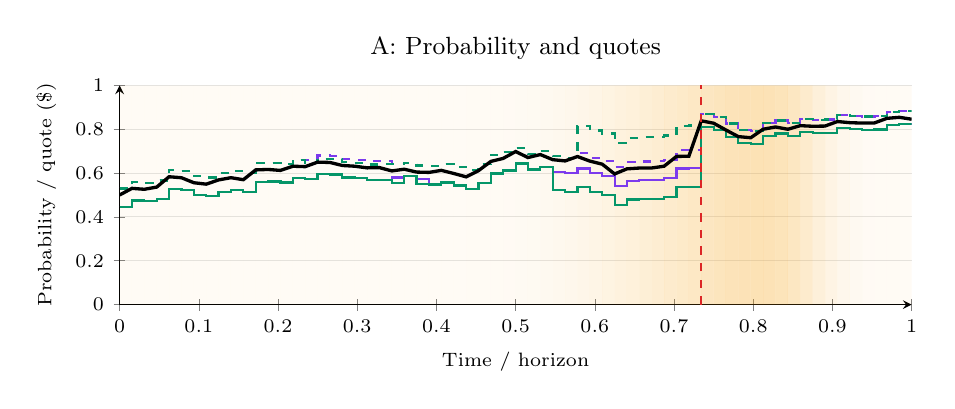
\begin{tikzpicture}
\begin{axis}[width=0.96\linewidth,height=0.36\linewidth,
xmin=0,xmax=1,ymin=0,ymax=1,axis lines=left,ymajorgrids,grid style={gray!20},
label style={font=\scriptsize},tick label style={font=\scriptsize},
title style={font=\small},title={A: Probability and quotes},
xlabel={Time / horizon},ylabel={Probability / quote (\$)}]
\addplot[draw=none,fill=prototypehazard,fill opacity=0.040000,forget plot] coordinates {(0.00000000,0.00000000) (0.01562500,0.00000000) (0.01562500,1.00000000) (0.00000000,1.00000000)} \closedcycle;
\addplot[draw=none,fill=prototypehazard,fill opacity=0.040000,forget plot] coordinates {(0.01562500,0.00000000) (0.03125000,0.00000000) (0.03125000,1.00000000) (0.01562500,1.00000000)} \closedcycle;
\addplot[draw=none,fill=prototypehazard,fill opacity=0.040000,forget plot] coordinates {(0.03125000,0.00000000) (0.04687500,0.00000000) (0.04687500,1.00000000) (0.03125000,1.00000000)} \closedcycle;
\addplot[draw=none,fill=prototypehazard,fill opacity=0.040000,forget plot] coordinates {(0.04687500,0.00000000) (0.06250000,0.00000000) (0.06250000,1.00000000) (0.04687500,1.00000000)} \closedcycle;
\addplot[draw=none,fill=prototypehazard,fill opacity=0.040000,forget plot] coordinates {(0.06250000,0.00000000) (0.07812500,0.00000000) (0.07812500,1.00000000) (0.06250000,1.00000000)} \closedcycle;
\addplot[draw=none,fill=prototypehazard,fill opacity=0.040000,forget plot] coordinates {(0.07812500,0.00000000) (0.09375000,0.00000000) (0.09375000,1.00000000) (0.07812500,1.00000000)} \closedcycle;
\addplot[draw=none,fill=prototypehazard,fill opacity=0.040000,forget plot] coordinates {(0.09375000,0.00000000) (0.10937500,0.00000000) (0.10937500,1.00000000) (0.09375000,1.00000000)} \closedcycle;
\addplot[draw=none,fill=prototypehazard,fill opacity=0.040000,forget plot] coordinates {(0.10937500,0.00000000) (0.12500000,0.00000000) (0.12500000,1.00000000) (0.10937500,1.00000000)} \closedcycle;
\addplot[draw=none,fill=prototypehazard,fill opacity=0.040000,forget plot] coordinates {(0.12500000,0.00000000) (0.14062500,0.00000000) (0.14062500,1.00000000) (0.12500000,1.00000000)} \closedcycle;
\addplot[draw=none,fill=prototypehazard,fill opacity=0.040000,forget plot] coordinates {(0.14062500,0.00000000) (0.15625000,0.00000000) (0.15625000,1.00000000) (0.14062500,1.00000000)} \closedcycle;
\addplot[draw=none,fill=prototypehazard,fill opacity=0.040000,forget plot] coordinates {(0.15625000,0.00000000) (0.17187500,0.00000000) (0.17187500,1.00000000) (0.15625000,1.00000000)} \closedcycle;
\addplot[draw=none,fill=prototypehazard,fill opacity=0.040000,forget plot] coordinates {(0.17187500,0.00000000) (0.18750000,0.00000000) (0.18750000,1.00000000) (0.17187500,1.00000000)} \closedcycle;
\addplot[draw=none,fill=prototypehazard,fill opacity=0.040000,forget plot] coordinates {(0.18750000,0.00000000) (0.20312500,0.00000000) (0.20312500,1.00000000) (0.18750000,1.00000000)} \closedcycle;
\addplot[draw=none,fill=prototypehazard,fill opacity=0.040000,forget plot] coordinates {(0.20312500,0.00000000) (0.21875000,0.00000000) (0.21875000,1.00000000) (0.20312500,1.00000000)} \closedcycle;
\addplot[draw=none,fill=prototypehazard,fill opacity=0.040000,forget plot] coordinates {(0.21875000,0.00000000) (0.23437500,0.00000000) (0.23437500,1.00000000) (0.21875000,1.00000000)} \closedcycle;
\addplot[draw=none,fill=prototypehazard,fill opacity=0.040000,forget plot] coordinates {(0.23437500,0.00000000) (0.25000000,0.00000000) (0.25000000,1.00000000) (0.23437500,1.00000000)} \closedcycle;
\addplot[draw=none,fill=prototypehazard,fill opacity=0.040000,forget plot] coordinates {(0.25000000,0.00000000) (0.26562500,0.00000000) (0.26562500,1.00000000) (0.25000000,1.00000000)} \closedcycle;
\addplot[draw=none,fill=prototypehazard,fill opacity=0.040000,forget plot] coordinates {(0.26562500,0.00000000) (0.28125000,0.00000000) (0.28125000,1.00000000) (0.26562500,1.00000000)} \closedcycle;
\addplot[draw=none,fill=prototypehazard,fill opacity=0.040001,forget plot] coordinates {(0.28125000,0.00000000) (0.29687500,0.00000000) (0.29687500,1.00000000) (0.28125000,1.00000000)} \closedcycle;
\addplot[draw=none,fill=prototypehazard,fill opacity=0.040002,forget plot] coordinates {(0.29687500,0.00000000) (0.31250000,0.00000000) (0.31250000,1.00000000) (0.29687500,1.00000000)} \closedcycle;
\addplot[draw=none,fill=prototypehazard,fill opacity=0.040004,forget plot] coordinates {(0.31250000,0.00000000) (0.32812500,0.00000000) (0.32812500,1.00000000) (0.31250000,1.00000000)} \closedcycle;
\addplot[draw=none,fill=prototypehazard,fill opacity=0.040009,forget plot] coordinates {(0.32812500,0.00000000) (0.34375000,0.00000000) (0.34375000,1.00000000) (0.32812500,1.00000000)} \closedcycle;
\addplot[draw=none,fill=prototypehazard,fill opacity=0.040022,forget plot] coordinates {(0.34375000,0.00000000) (0.35937500,0.00000000) (0.35937500,1.00000000) (0.34375000,1.00000000)} \closedcycle;
\addplot[draw=none,fill=prototypehazard,fill opacity=0.040050,forget plot] coordinates {(0.35937500,0.00000000) (0.37500000,0.00000000) (0.37500000,1.00000000) (0.35937500,1.00000000)} \closedcycle;
\addplot[draw=none,fill=prototypehazard,fill opacity=0.040106,forget plot] coordinates {(0.37500000,0.00000000) (0.39062500,0.00000000) (0.39062500,1.00000000) (0.37500000,1.00000000)} \closedcycle;
\addplot[draw=none,fill=prototypehazard,fill opacity=0.040219,forget plot] coordinates {(0.39062500,0.00000000) (0.40625000,0.00000000) (0.40625000,1.00000000) (0.39062500,1.00000000)} \closedcycle;
\addplot[draw=none,fill=prototypehazard,fill opacity=0.040431,forget plot] coordinates {(0.40625000,0.00000000) (0.42187500,0.00000000) (0.42187500,1.00000000) (0.40625000,1.00000000)} \closedcycle;
\addplot[draw=none,fill=prototypehazard,fill opacity=0.040812,forget plot] coordinates {(0.42187500,0.00000000) (0.43750000,0.00000000) (0.43750000,1.00000000) (0.42187500,1.00000000)} \closedcycle;
\addplot[draw=none,fill=prototypehazard,fill opacity=0.041467,forget plot] coordinates {(0.43750000,0.00000000) (0.45312500,0.00000000) (0.45312500,1.00000000) (0.43750000,1.00000000)} \closedcycle;
\addplot[draw=none,fill=prototypehazard,fill opacity=0.042540,forget plot] coordinates {(0.45312500,0.00000000) (0.46875000,0.00000000) (0.46875000,1.00000000) (0.45312500,1.00000000)} \closedcycle;
\addplot[draw=none,fill=prototypehazard,fill opacity=0.044218,forget plot] coordinates {(0.46875000,0.00000000) (0.48437500,0.00000000) (0.48437500,1.00000000) (0.46875000,1.00000000)} \closedcycle;
\addplot[draw=none,fill=prototypehazard,fill opacity=0.046720,forget plot] coordinates {(0.48437500,0.00000000) (0.50000000,0.00000000) (0.50000000,1.00000000) (0.48437500,1.00000000)} \closedcycle;
\addplot[draw=none,fill=prototypehazard,fill opacity=0.050288,forget plot] coordinates {(0.50000000,0.00000000) (0.51562500,0.00000000) (0.51562500,1.00000000) (0.50000000,1.00000000)} \closedcycle;
\addplot[draw=none,fill=prototypehazard,fill opacity=0.055156,forget plot] coordinates {(0.51562500,0.00000000) (0.53125000,0.00000000) (0.53125000,1.00000000) (0.51562500,1.00000000)} \closedcycle;
\addplot[draw=none,fill=prototypehazard,fill opacity=0.061525,forget plot] coordinates {(0.53125000,0.00000000) (0.54687500,0.00000000) (0.54687500,1.00000000) (0.53125000,1.00000000)} \closedcycle;
\addplot[draw=none,fill=prototypehazard,fill opacity=0.069533,forget plot] coordinates {(0.54687500,0.00000000) (0.56250000,0.00000000) (0.56250000,1.00000000) (0.54687500,1.00000000)} \closedcycle;
\addplot[draw=none,fill=prototypehazard,fill opacity=0.079241,forget plot] coordinates {(0.56250000,0.00000000) (0.57812500,0.00000000) (0.57812500,1.00000000) (0.56250000,1.00000000)} \closedcycle;
\addplot[draw=none,fill=prototypehazard,fill opacity=0.090626,forget plot] coordinates {(0.57812500,0.00000000) (0.59375000,0.00000000) (0.59375000,1.00000000) (0.57812500,1.00000000)} \closedcycle;
\addplot[draw=none,fill=prototypehazard,fill opacity=0.103585,forget plot] coordinates {(0.59375000,0.00000000) (0.60937500,0.00000000) (0.60937500,1.00000000) (0.59375000,1.00000000)} \closedcycle;
\addplot[draw=none,fill=prototypehazard,fill opacity=0.117952,forget plot] coordinates {(0.60937500,0.00000000) (0.62500000,0.00000000) (0.62500000,1.00000000) (0.60937500,1.00000000)} \closedcycle;
\addplot[draw=none,fill=prototypehazard,fill opacity=0.133515,forget plot] coordinates {(0.62500000,0.00000000) (0.64062500,0.00000000) (0.64062500,1.00000000) (0.62500000,1.00000000)} \closedcycle;
\addplot[draw=none,fill=prototypehazard,fill opacity=0.150038,forget plot] coordinates {(0.64062500,0.00000000) (0.65625000,0.00000000) (0.65625000,1.00000000) (0.64062500,1.00000000)} \closedcycle;
\addplot[draw=none,fill=prototypehazard,fill opacity=0.167274,forget plot] coordinates {(0.65625000,0.00000000) (0.67187500,0.00000000) (0.67187500,1.00000000) (0.65625000,1.00000000)} \closedcycle;
\addplot[draw=none,fill=prototypehazard,fill opacity=0.184975,forget plot] coordinates {(0.67187500,0.00000000) (0.68750000,0.00000000) (0.68750000,1.00000000) (0.67187500,1.00000000)} \closedcycle;
\addplot[draw=none,fill=prototypehazard,fill opacity=0.202890,forget plot] coordinates {(0.68750000,0.00000000) (0.70312500,0.00000000) (0.70312500,1.00000000) (0.68750000,1.00000000)} \closedcycle;
\addplot[draw=none,fill=prototypehazard,fill opacity=0.220762,forget plot] coordinates {(0.70312500,0.00000000) (0.71875000,0.00000000) (0.71875000,1.00000000) (0.70312500,1.00000000)} \closedcycle;
\addplot[draw=none,fill=prototypehazard,fill opacity=0.238300,forget plot] coordinates {(0.71875000,0.00000000) (0.73437500,0.00000000) (0.73437500,1.00000000) (0.71875000,1.00000000)} \closedcycle;
\addplot[draw=none,fill=prototypehazard,fill opacity=0.255144,forget plot] coordinates {(0.73437500,0.00000000) (0.75000000,0.00000000) (0.75000000,1.00000000) (0.73437500,1.00000000)} \closedcycle;
\addplot[draw=none,fill=prototypehazard,fill opacity=0.270787,forget plot] coordinates {(0.75000000,0.00000000) (0.76562500,0.00000000) (0.76562500,1.00000000) (0.75000000,1.00000000)} \closedcycle;
\addplot[draw=none,fill=prototypehazard,fill opacity=0.284449,forget plot] coordinates {(0.76562500,0.00000000) (0.78125000,0.00000000) (0.78125000,1.00000000) (0.76562500,1.00000000)} \closedcycle;
\addplot[draw=none,fill=prototypehazard,fill opacity=0.294868,forget plot] coordinates {(0.78125000,0.00000000) (0.79687500,0.00000000) (0.79687500,1.00000000) (0.78125000,1.00000000)} \closedcycle;
\addplot[draw=none,fill=prototypehazard,fill opacity=0.300000,forget plot] coordinates {(0.79687500,0.00000000) (0.81250000,0.00000000) (0.81250000,1.00000000) (0.79687500,1.00000000)} \closedcycle;
\addplot[draw=none,fill=prototypehazard,fill opacity=0.296731,forget plot] coordinates {(0.81250000,0.00000000) (0.82812500,0.00000000) (0.82812500,1.00000000) (0.81250000,1.00000000)} \closedcycle;
\addplot[draw=none,fill=prototypehazard,fill opacity=0.281065,forget plot] coordinates {(0.82812500,0.00000000) (0.84375000,0.00000000) (0.84375000,1.00000000) (0.82812500,1.00000000)} \closedcycle;
\addplot[draw=none,fill=prototypehazard,fill opacity=0.249827,forget plot] coordinates {(0.84375000,0.00000000) (0.85937500,0.00000000) (0.85937500,1.00000000) (0.84375000,1.00000000)} \closedcycle;
\addplot[draw=none,fill=prototypehazard,fill opacity=0.204419,forget plot] coordinates {(0.85937500,0.00000000) (0.87500000,0.00000000) (0.87500000,1.00000000) (0.85937500,1.00000000)} \closedcycle;
\addplot[draw=none,fill=prototypehazard,fill opacity=0.153498,forget plot] coordinates {(0.87500000,0.00000000) (0.89062500,0.00000000) (0.89062500,1.00000000) (0.87500000,1.00000000)} \closedcycle;
\addplot[draw=none,fill=prototypehazard,fill opacity=0.108844,forget plot] coordinates {(0.89062500,0.00000000) (0.90625000,0.00000000) (0.90625000,1.00000000) (0.89062500,1.00000000)} \closedcycle;
\addplot[draw=none,fill=prototypehazard,fill opacity=0.077292,forget plot] coordinates {(0.90625000,0.00000000) (0.92187500,0.00000000) (0.92187500,1.00000000) (0.90625000,1.00000000)} \closedcycle;
\addplot[draw=none,fill=prototypehazard,fill opacity=0.058465,forget plot] coordinates {(0.92187500,0.00000000) (0.93750000,0.00000000) (0.93750000,1.00000000) (0.92187500,1.00000000)} \closedcycle;
\addplot[draw=none,fill=prototypehazard,fill opacity=0.048523,forget plot] coordinates {(0.93750000,0.00000000) (0.95312500,0.00000000) (0.95312500,1.00000000) (0.93750000,1.00000000)} \closedcycle;
\addplot[draw=none,fill=prototypehazard,fill opacity=0.043715,forget plot] coordinates {(0.95312500,0.00000000) (0.96875000,0.00000000) (0.96875000,1.00000000) (0.95312500,1.00000000)} \closedcycle;
\addplot[draw=none,fill=prototypehazard,fill opacity=0.041541,forget plot] coordinates {(0.96875000,0.00000000) (0.98437500,0.00000000) (0.98437500,1.00000000) (0.96875000,1.00000000)} \closedcycle;
\addplot[draw=none,fill=prototypehazard,fill opacity=0.040610,forget plot] coordinates {(0.98437500,0.00000000) (1.00000000,0.00000000) (1.00000000,1.00000000) (0.98437500,1.00000000)} \closedcycle;
\addplot[prototypeoriginal,const plot,thick] coordinates {(0.00000000,0.44500000) (0.01562500,0.47535934) (0.03125000,0.47112306) (0.04687500,0.48114863) (0.06250000,0.52831439) (0.07812500,0.52383942) (0.09375000,0.50101744) (0.10937500,0.49449551) (0.12500000,0.51388923) (0.14062500,0.52397138) (0.15625000,0.51485288) (0.17187500,0.55957676) (0.18750000,0.56157096) (0.20312500,0.55720487) (0.21875000,0.57633170) (0.23437500,0.57436431) (0.25000000,0.59503586) (0.26562500,0.59345889) (0.28125000,0.57970076) (0.29687500,0.57637094) (0.31250000,0.56889894) (0.32812500,0.56992801) (0.34375000,0.57983702) (0.35937500,0.58763320) (0.37500000,0.57463774) (0.39062500,0.54813908) (0.40625000,0.55740340) (0.42187500,0.54327451) (0.43750000,0.52788967) (0.45312500,0.55609183) (0.46875000,0.59824056) (0.48437500,0.61216279) (0.50000000,0.64332582) (0.51562500,0.61600298) (0.53125000,0.62949266) (0.54687500,0.60623664) (0.56250000,0.60048097) (0.57812500,0.62055946) (0.59375000,0.59966034) (0.60937500,0.58560290) (0.62500000,0.54111211) (0.64062500,0.56439629) (0.65625000,0.56807454) (0.67187500,0.56838846) (0.68750000,0.57638006) (0.70312500,0.62100313) (0.71875000,0.62200324) (0.73437500,0.80850162) (0.75000000,0.79758464) (0.76562500,0.76637877) (0.78125000,0.73642307) (0.79687500,0.73128734) (0.81250000,0.77013441) (0.82812500,0.78038370) (0.84375000,0.77000769) (0.85937500,0.78636449) (0.87500000,0.78364732) (0.89062500,0.78449836) (0.90625000,0.80521584) (0.92187500,0.80008924) (0.93750000,0.79814974) (0.95312500,0.79888935) (0.96875000,0.81970586) (0.98437500,0.82447722) (1.00000000,0.82447722)};
\addplot[prototypeoriginal,const plot,thick,dashed] coordinates {(0.00000000,0.53000000) (0.01562500,0.56035934) (0.03125000,0.55612306) (0.04687500,0.56614863) (0.06250000,0.61331439) (0.07812500,0.60883942) (0.09375000,0.58601744) (0.10937500,0.57949551) (0.12500000,0.59888923) (0.14062500,0.60897138) (0.15625000,0.59985288) (0.17187500,0.64457676) (0.18750000,0.64657096) (0.20312500,0.64220487) (0.21875000,0.66133170) (0.23437500,0.65936431) (0.25000000,0.68003586) (0.26562500,0.67845889) (0.28125000,0.66470076) (0.29687500,0.66137094) (0.31250000,0.65389894) (0.32812500,0.65492801) (0.34375000,0.63983702) (0.35937500,0.64763320) (0.37500000,0.63463774) (0.39062500,0.63313908) (0.40625000,0.64240340) (0.42187500,0.62827451) (0.43750000,0.61288967) (0.45312500,0.64109183) (0.46875000,0.68324056) (0.48437500,0.69716279) (0.50000000,0.71332582) (0.51562500,0.68600298) (0.53125000,0.69949266) (0.54687500,0.67623664) (0.56250000,0.67048097) (0.57812500,0.69055946) (0.59375000,0.66966034) (0.60937500,0.65560290) (0.62500000,0.62611211) (0.64062500,0.64939629) (0.65625000,0.65307454) (0.67187500,0.65338846) (0.68750000,0.66138006) (0.70312500,0.70600313) (0.71875000,0.70700324) (0.73437500,0.86850162) (0.75000000,0.85758464) (0.76562500,0.82637877) (0.78125000,0.79642307) (0.79687500,0.79128734) (0.81250000,0.83013441) (0.82812500,0.84038370) (0.84375000,0.83000769) (0.85937500,0.84636449) (0.87500000,0.84364732) (0.89062500,0.84449836) (0.90625000,0.86521584) (0.92187500,0.86008924) (0.93750000,0.85814974) (0.95312500,0.85888935) (0.96875000,0.87970586) (0.98437500,0.88447722) (1.00000000,0.88447722)};
\addplot[prototypeaware,const plot,thick] coordinates {(0.00000000,0.44500000) (0.01562500,0.47535934) (0.03125000,0.47112306) (0.04687500,0.48114863) (0.06250000,0.52831439) (0.07812500,0.52383942) (0.09375000,0.50101744) (0.10937500,0.49449551) (0.12500000,0.51388923) (0.14062500,0.52397138) (0.15625000,0.51485288) (0.17187500,0.55957676) (0.18750000,0.56157096) (0.20312500,0.55720487) (0.21875000,0.57633170) (0.23437500,0.57436431) (0.25000000,0.59503586) (0.26562500,0.59345889) (0.28125000,0.57970076) (0.29687500,0.57637094) (0.31250000,0.56889894) (0.32812500,0.56992801) (0.34375000,0.55483702) (0.35937500,0.58763320) (0.37500000,0.54963774) (0.39062500,0.54813908) (0.40625000,0.55740340) (0.42187500,0.54327451) (0.43750000,0.52788967) (0.45312500,0.55609183) (0.46875000,0.59824056) (0.48437500,0.61216279) (0.50000000,0.64332582) (0.51562500,0.61600298) (0.53125000,0.62949266) (0.54687500,0.52123664) (0.56250000,0.51548097) (0.57812500,0.53555946) (0.59375000,0.51466034) (0.60937500,0.50060290) (0.62500000,0.45611211) (0.64062500,0.47939629) (0.65625000,0.48307454) (0.67187500,0.48338846) (0.68750000,0.49138006) (0.70312500,0.53600313) (0.71875000,0.53700324) (0.73437500,0.80850162) (0.75000000,0.79758464) (0.76562500,0.76637877) (0.78125000,0.73642307) (0.79687500,0.73128734) (0.81250000,0.77013441) (0.82812500,0.78038370) (0.84375000,0.77000769) (0.85937500,0.78636449) (0.87500000,0.78364732) (0.89062500,0.78449836) (0.90625000,0.80521584) (0.92187500,0.80008924) (0.93750000,0.79814974) (0.95312500,0.79888935) (0.96875000,0.81970586) (0.98437500,0.82447722) (1.00000000,0.82447722)};
\addplot[prototypeaware,const plot,thick,dashed] coordinates {(0.00000000,0.53000000) (0.01562500,0.56035934) (0.03125000,0.55612306) (0.04687500,0.56614863) (0.06250000,0.61331439) (0.07812500,0.60883942) (0.09375000,0.58601744) (0.10937500,0.57949551) (0.12500000,0.59888923) (0.14062500,0.60897138) (0.15625000,0.59985288) (0.17187500,0.64457676) (0.18750000,0.64657096) (0.20312500,0.64220487) (0.21875000,0.66133170) (0.23437500,0.64436431) (0.25000000,0.66503586) (0.26562500,0.66345889) (0.28125000,0.64970076) (0.29687500,0.64637094) (0.31250000,0.63889894) (0.32812500,0.63992801) (0.34375000,0.63983702) (0.35937500,0.64763320) (0.37500000,0.63463774) (0.39062500,0.63313908) (0.40625000,0.64240340) (0.42187500,0.62827451) (0.43750000,0.61288967) (0.45312500,0.64109183) (0.46875000,0.68324056) (0.48437500,0.69716279) (0.50000000,0.71332582) (0.51562500,0.68600298) (0.53125000,0.69949266) (0.54687500,0.67623664) (0.56250000,0.67048097) (0.57812500,0.81555946) (0.59375000,0.79466034) (0.60937500,0.78060290) (0.62500000,0.73611211) (0.64062500,0.75939629) (0.65625000,0.76307454) (0.67187500,0.76338846) (0.68750000,0.77138006) (0.70312500,0.81600313) (0.71875000,0.81700324) (0.73437500,0.86850162) (0.75000000,0.85758464) (0.76562500,0.82637877) (0.78125000,0.79642307) (0.79687500,0.79128734) (0.81250000,0.83013441) (0.82812500,0.84038370) (0.84375000,0.83000769) (0.85937500,0.84636449) (0.87500000,0.84364732) (0.89062500,0.84449836) (0.90625000,0.86521584) (0.92187500,0.86008924) (0.93750000,0.85814974) (0.95312500,0.85888935) (0.96875000,0.87970586) (0.98437500,0.88447722) (1.00000000,0.88447722)};
\addplot[black,very thick] coordinates {(0.00000000,0.50000000) (0.01562500,0.53035934) (0.03125000,0.52612306) (0.04687500,0.53614863) (0.06250000,0.58331439) (0.07812500,0.57883942) (0.09375000,0.55601744) (0.10937500,0.54949551) (0.12500000,0.56888923) (0.14062500,0.57897138) (0.15625000,0.56985288) (0.17187500,0.61457676) (0.18750000,0.61657096) (0.20312500,0.61220487) (0.21875000,0.63133170) (0.23437500,0.62936431) (0.25000000,0.65003586) (0.26562500,0.64845889) (0.28125000,0.63470076) (0.29687500,0.63137094) (0.31250000,0.62389894) (0.32812500,0.62492801) (0.34375000,0.60983702) (0.35937500,0.61763320) (0.37500000,0.60463774) (0.39062500,0.60313908) (0.40625000,0.61240340) (0.42187500,0.59827451) (0.43750000,0.58288967) (0.45312500,0.61109183) (0.46875000,0.65324056) (0.48437500,0.66716279) (0.50000000,0.69832582) (0.51562500,0.67100298) (0.53125000,0.68449266) (0.54687500,0.66123664) (0.56250000,0.65548097) (0.57812500,0.67555946) (0.59375000,0.65466034) (0.60937500,0.64060290) (0.62500000,0.59611211) (0.64062500,0.61939629) (0.65625000,0.62307454) (0.67187500,0.62338846) (0.68750000,0.63138006) (0.70312500,0.67600313) (0.71875000,0.67700324) (0.73437500,0.83850162) (0.75000000,0.82758464) (0.76562500,0.79637877) (0.78125000,0.76642307) (0.79687500,0.76128734) (0.81250000,0.80013441) (0.82812500,0.81038370) (0.84375000,0.80000769) (0.85937500,0.81636449) (0.87500000,0.81364732) (0.89062500,0.81449836) (0.90625000,0.83521584) (0.92187500,0.83008924) (0.93750000,0.82814974) (0.95312500,0.82888935) (0.96875000,0.84970586) (0.98437500,0.85447722) (1.00000000,0.84580126)};
\addplot[prototypeevent,dashed,thick,forget plot] coordinates {(0.73437500,0.00000000) (0.73437500,1.00000000)};
\end{axis}\end{tikzpicture}
\par\bigskip
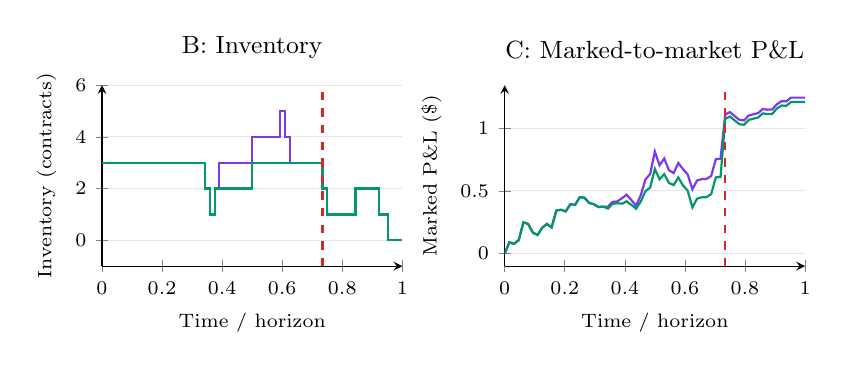
\begin{tikzpicture}
\begin{groupplot}[group style={group size=2 by 1,horizontal sep=1.3cm},
width=0.445\linewidth,height=0.32\linewidth,
xmin=0,xmax=1,axis lines=left,ymajorgrids,grid style={gray!20},
label style={font=\scriptsize},tick label style={font=\scriptsize},
title style={font=\small}]
\nextgroupplot[title={B: Inventory},xlabel={Time / horizon},ylabel={Inventory (contracts)}]
\addplot[prototypeoriginal,const plot,thick] coordinates {(0.00000000,3.00000000) (0.01562500,3.00000000) (0.03125000,3.00000000) (0.04687500,3.00000000) (0.06250000,3.00000000) (0.07812500,3.00000000) (0.09375000,3.00000000) (0.10937500,3.00000000) (0.12500000,3.00000000) (0.14062500,3.00000000) (0.15625000,3.00000000) (0.17187500,3.00000000) (0.18750000,3.00000000) (0.20312500,3.00000000) (0.21875000,3.00000000) (0.23437500,3.00000000) (0.25000000,3.00000000) (0.26562500,3.00000000) (0.28125000,3.00000000) (0.29687500,3.00000000) (0.31250000,3.00000000) (0.32812500,3.00000000) (0.34375000,2.00000000) (0.35937500,1.00000000) (0.37500000,2.00000000) (0.39062500,3.00000000) (0.40625000,3.00000000) (0.42187500,3.00000000) (0.43750000,3.00000000) (0.45312500,3.00000000) (0.46875000,3.00000000) (0.48437500,3.00000000) (0.50000000,4.00000000) (0.51562500,4.00000000) (0.53125000,4.00000000) (0.54687500,4.00000000) (0.56250000,4.00000000) (0.57812500,4.00000000) (0.59375000,5.00000000) (0.60937500,4.00000000) (0.62500000,3.00000000) (0.64062500,3.00000000) (0.65625000,3.00000000) (0.67187500,3.00000000) (0.68750000,3.00000000) (0.70312500,3.00000000) (0.71875000,3.00000000) (0.73437500,2.00000000) (0.75000000,1.00000000) (0.76562500,1.00000000) (0.78125000,1.00000000) (0.79687500,1.00000000) (0.81250000,1.00000000) (0.82812500,1.00000000) (0.84375000,2.00000000) (0.85937500,2.00000000) (0.87500000,2.00000000) (0.89062500,2.00000000) (0.90625000,2.00000000) (0.92187500,1.00000000) (0.93750000,1.00000000) (0.95312500,0.00000000) (0.96875000,0.00000000) (0.98437500,0.00000000) (1.00000000,0.00000000)};
\addplot[prototypeaware,const plot,thick] coordinates {(0.00000000,3.00000000) (0.01562500,3.00000000) (0.03125000,3.00000000) (0.04687500,3.00000000) (0.06250000,3.00000000) (0.07812500,3.00000000) (0.09375000,3.00000000) (0.10937500,3.00000000) (0.12500000,3.00000000) (0.14062500,3.00000000) (0.15625000,3.00000000) (0.17187500,3.00000000) (0.18750000,3.00000000) (0.20312500,3.00000000) (0.21875000,3.00000000) (0.23437500,3.00000000) (0.25000000,3.00000000) (0.26562500,3.00000000) (0.28125000,3.00000000) (0.29687500,3.00000000) (0.31250000,3.00000000) (0.32812500,3.00000000) (0.34375000,2.00000000) (0.35937500,1.00000000) (0.37500000,2.00000000) (0.39062500,2.00000000) (0.40625000,2.00000000) (0.42187500,2.00000000) (0.43750000,2.00000000) (0.45312500,2.00000000) (0.46875000,2.00000000) (0.48437500,2.00000000) (0.50000000,3.00000000) (0.51562500,3.00000000) (0.53125000,3.00000000) (0.54687500,3.00000000) (0.56250000,3.00000000) (0.57812500,3.00000000) (0.59375000,3.00000000) (0.60937500,3.00000000) (0.62500000,3.00000000) (0.64062500,3.00000000) (0.65625000,3.00000000) (0.67187500,3.00000000) (0.68750000,3.00000000) (0.70312500,3.00000000) (0.71875000,3.00000000) (0.73437500,2.00000000) (0.75000000,1.00000000) (0.76562500,1.00000000) (0.78125000,1.00000000) (0.79687500,1.00000000) (0.81250000,1.00000000) (0.82812500,1.00000000) (0.84375000,2.00000000) (0.85937500,2.00000000) (0.87500000,2.00000000) (0.89062500,2.00000000) (0.90625000,2.00000000) (0.92187500,1.00000000) (0.93750000,1.00000000) (0.95312500,0.00000000) (0.96875000,0.00000000) (0.98437500,0.00000000) (1.00000000,0.00000000)};
\addplot[prototypeevent,dashed,thick,forget plot] coordinates {(0.73437500,-1.00000000) (0.73437500,6.00000000)};
\nextgroupplot[title={C: Marked-to-market P\&L},xlabel={Time / horizon},ylabel={Marked P\&L (\$)}]
\addplot[prototypeoriginal,thick] coordinates {(0.00000000,0.00000000) (0.01562500,0.09107803) (0.03125000,0.07836918) (0.04687500,0.10844588) (0.06250000,0.24994318) (0.07812500,0.23651825) (0.09375000,0.16805231) (0.10937500,0.14848654) (0.12500000,0.20666769) (0.14062500,0.23691413) (0.15625000,0.20955864) (0.17187500,0.34373029) (0.18750000,0.34971289) (0.20312500,0.33661462) (0.21875000,0.39399510) (0.23437500,0.38809293) (0.25000000,0.45010757) (0.26562500,0.44537668) (0.28125000,0.40410228) (0.29687500,0.39411283) (0.31250000,0.37169682) (0.32812500,0.37478403) (0.34375000,0.37460206) (0.35937500,0.41239823) (0.37500000,0.41640731) (0.39062500,0.44191132) (0.40625000,0.46970430) (0.42187500,0.42731764) (0.43750000,0.38116310) (0.45312500,0.46576959) (0.46875000,0.59221578) (0.48437500,0.63398248) (0.50000000,0.81363460) (0.51562500,0.70434324) (0.53125000,0.75830196) (0.54687500,0.66527786) (0.56250000,0.64225516) (0.57812500,0.72256914) (0.59375000,0.67307354) (0.60937500,0.63184380) (0.62500000,0.51337142) (0.64062500,0.58322396) (0.65625000,0.59425870) (0.67187500,0.59520048) (0.68750000,0.61917527) (0.70312500,0.75304447) (0.71875000,0.75604480) (0.73437500,1.10904156) (0.75000000,1.12812458) (0.76562500,1.09691872) (0.78125000,1.06696301) (0.79687500,1.06182728) (0.81250000,1.10067435) (0.82812500,1.11092364) (0.84375000,1.12017163) (0.85937500,1.15288523) (0.87500000,1.14745088) (0.89062500,1.14915295) (0.90625000,1.19058792) (0.92187500,1.21546132) (0.93750000,1.21352182) (0.95312500,1.24352182) (0.96875000,1.24352182) (0.98437500,1.24352182) (1.00000000,1.24352182)};
\addplot[prototypeaware,thick] coordinates {(0.00000000,0.00000000) (0.01562500,0.09107803) (0.03125000,0.07836918) (0.04687500,0.10844588) (0.06250000,0.24994318) (0.07812500,0.23651825) (0.09375000,0.16805231) (0.10937500,0.14848654) (0.12500000,0.20666769) (0.14062500,0.23691413) (0.15625000,0.20955864) (0.17187500,0.34373029) (0.18750000,0.34971289) (0.20312500,0.33661462) (0.21875000,0.39399510) (0.23437500,0.38809293) (0.25000000,0.45010757) (0.26562500,0.44537668) (0.28125000,0.40410228) (0.29687500,0.39411283) (0.31250000,0.37169682) (0.32812500,0.37478403) (0.34375000,0.35960206) (0.35937500,0.39739823) (0.37500000,0.40140731) (0.39062500,0.39840999) (0.40625000,0.41693863) (0.42187500,0.38868086) (0.43750000,0.35791117) (0.45312500,0.41431549) (0.46875000,0.49861296) (0.48437500,0.52645742) (0.50000000,0.67494651) (0.51562500,0.59297799) (0.53125000,0.63344703) (0.54687500,0.56367896) (0.56250000,0.54641194) (0.57812500,0.60664742) (0.59375000,0.54395006) (0.60937500,0.50177775) (0.62500000,0.36830537) (0.64062500,0.43815791) (0.65625000,0.44919265) (0.67187500,0.45013443) (0.68750000,0.47410922) (0.70312500,0.60797843) (0.71875000,0.61097875) (0.73437500,1.07397551) (0.75000000,1.09305854) (0.76562500,1.06185267) (0.78125000,1.03189696) (0.79687500,1.02676123) (0.81250000,1.06560831) (0.82812500,1.07585760) (0.84375000,1.08510558) (0.85937500,1.11781918) (0.87500000,1.11238484) (0.89062500,1.11408691) (0.90625000,1.15552187) (0.92187500,1.18039527) (0.93750000,1.17845577) (0.95312500,1.20845577) (0.96875000,1.20845577) (0.98437500,1.20845577) (1.00000000,1.20845577)};
\addplot[prototypeevent,dashed,thick,forget plot] coordinates {(0.73437500,-0.09948175) (0.73437500,1.34300357)};
\end{groupplot}\end{tikzpicture}
\caption{Reproduction of the three interactive-prototype charts at default
settings and seed 2718. The upper panel shows fair probability and both
policies' bids and asks; the lower panels show inventory and marked P\&L.
Quotes are plotted at the start of each holding interval; inventory and P\&L
are plotted after each transition, with their initial values included. The
vertical red line marks the realized anticipated event. These physical-time
conventions replace the web page's common index-based horizontal scale.
The full terminal probability is included; the interactive plot truncates its
last probability observation. Colors reproduce the prototype's light theme.}
\label{fig:prototype}
\end{figure}

This illustration preserves the prototype's numerical behavior. It is a
separate configuration from the validated Monte Carlo comparison above. In
particular, the prototype clips probabilities to $[0.05,0.95]$, uses nearest-node
continuation values, and has different ordinary-fill approximations in its
Bellman recursion and its simulator. Its figures should therefore be read as
an illustration of that supplied implementation. They do not extend the main
experiment's Bellman-value validation or grid-refinement conclusions.
Exact replay data, default settings, and source hashes are saved in
\path{results/prototype_path.json}; reproduction scripts are
\path{simulation/reproduce_prototype.mjs} and
\path{simulation/prototype_report.py}.

% END GENERATED PROTOTYPE CHARTS
\clearpage
\appendix
\section{Optional partial-pickoff extension}
The baseline sets pickoff probability to one. For $0\le\chi\le1$, an independent
Bernoulli pickoff decision conditional on a crossing gives
\begin{equation}
 \G^{K,\chi}_{b,a}[W]
 =\chi\G^K_{b,a}[W]+(1-\chi)\int W(t,p',q)K(\dd p'\mid p).
\end{equation}
This mixes continuation inventories as well as markout losses. Merely
multiplying the loss term by $\chi$ while always changing inventory would be
inconsistent. The probability process and its risk charge are unchanged.
Certain pickoff is a maximal execution-probability case; it is not automatically
a bound on optimized total value because inventory effects also change.

\section{Specification status and provenance}
The shared discussion is the immediate source for this specification;
Section~\ref{sec:prior} identifies its published foundations and empirical
motivation. The event kernels, stale-event operator, coupled Bellman equations,
deterministic event interface, and experimental comparison are presented here
as the proposed framework. This write-up supplies explicit
admissibility and timing conventions, qualifies the spread result, and corrects
the unconditional variance-matching expression for one-shot survival. Numerical
parameters, participation limits, inventory limits, and grid resolution are
explicitly fixed for the synthetic experiment in Section~\ref{sec:mc}. Its
results are numerical model comparisons, without empirical calibration.
Bibliographic details and the limited empirical claims in Section~\ref{sec:prior}
were checked against the cited papers or their publisher/institutional records.
The bibliography distinguishes the direct foundation from contextual work;
it is not an exhaustive literature review.

\begin{thebibliography}{9}
\bibitem{feilnendel2026}
Dominik Feil and Max Nendel.
\newblock \emph{Optimal Market Making in Prediction Markets}.
\newblock arXiv preprint arXiv:2607.17991, 2026.
\newblock \url{https://arxiv.org/abs/2607.17991}.

\bibitem{avellanedastoikov2008}
Marco Avellaneda and Sasha Stoikov.
\newblock High-frequency trading in a limit order book.
\newblock \emph{Quantitative Finance}, 8(3):217--224, 2008.
\newblock \url{https://doi.org/10.1080/14697680701381228}.

\bibitem{cartea2015}
\'{A}lvaro Cartea, Sebastian Jaimungal, and Jos\'{e} Penalva.
\newblock \emph{Algorithmic and High-Frequency Trading}.
\newblock Cambridge University Press, 2015. ISBN 978-1-107-09114-6.
\newblock \href{https://assets.cambridge.org/97811070/91146/frontmatter/9781107091146_frontmatter.pdf}{Publisher front matter and contents}.

\bibitem{frinohill2001}
Alex Frino and Amelia Hill.
\newblock Intraday futures market behaviour around major scheduled
macroeconomic announcements: Australian evidence.
\newblock \emph{Journal of Banking \& Finance}, 25(7):1319--1337, 2001.
\newblock \url{https://doi.org/10.1016/S0378-4266(00)00132-1}.

\bibitem{siikanen2017}
Milla Siikanen, Juho Kanniainen, and Jaakko Valli.
\newblock Limit order books and liquidity around scheduled and non-scheduled
announcements: Empirical evidence from NASDAQ Nordic.
\newblock \emph{Finance Research Letters}, 21:264--271, 2017.
\newblock \url{https://doi.org/10.1016/j.frl.2016.12.016}.
\end{thebibliography}
\end{document}
